% 第 3 章：高阶乘积
\chapter{高阶乘积}\label{ch:higher-products}
上一章中，我们看到，在上同调环上定义高阶乘积很有意义，因为取上同调的过程会丢失一些信息。本章将介绍由 Stasheff 最初发展的 $A_\infty$ 形式体系\bookcite{229}，它以协调一致的方式处理这些高阶乘积。随后，我们把这套形式体系与第一章的范畴论和表示论结合起来。最后还会考察这些思想的一些有用推广。

更多细节和背景材料可参见 Keller 的综述文章\bookcite{133}、\bookcite{135}，Seidel 著作的第一部分\bookcite{218}，以及 Kontsevich 与 Soibelman 的专著\bookcite{150}。

\section{动机与定义}\label{sec:ainfty-motivation}
\takeaway{微分、乘法与 Leibniz 律都是“两个运算复合后相消”的实例，可用根树统一图示；$A_\infty$ 代数把这三条恒等式推广为 $b_i\colon A[1]^{\otimes i}\to A[1]$ 上的一族 Stasheff 恒等式，$A_\infty$ 态射容许不同阶乘积混合；Koszul 符号是使 $\mu$ 与 $m$ 两种约定等价的枢纽。}
\subsection{推广结合律}\label{subsec:generalizing-associativity}
先考察此前遇到过的三种代数对象。上链复形是一个分次向量空间 $V$，带有一个次数为 $1$ 的一元运算 $\delta$，满足微分律 $\delta^2=0$。分次代数 $R$ 是一个分次向量空间，带有一个次数为 $0$ 的二元运算“$\cdot$”，满足结合律。第三种对象是 dg-代数，它同时具有这两种运算。每种运算各自满足相应恒等式，二者还须满足一条额外规律：分次 Leibniz 律。为了避免陷入符号细节，我们暂时假设工作域 $k$ 的特征为 $2$，并给出这三种看似不同的规律的一种统一解释。
% [Tutor Note: 假设 $\mathrm{char}\,k=2$ 时 $+1=-1$，所以下面三条恒等式里的所有符号都消失了；在特征 $0$ 的域上，须改用带 Koszul 符号的 $b_k$（见 §3.1.4），三条恒等式才严格成立。切勿把特征 $2$ 下的“统一解释”直接搬到特征 $0$。]

将恒等映射记作 $1$，令
\[
  \mu_1\colon V\to V,\quad v\longmapsto\delta v,
\qquad
  \mu_2\colon V^{\otimes2}\to V,\quad
  v\otimes w\longmapsto v\cdot w.
\]
于是三条规律可以写成
\begin{align*}
  [\mathrm{DIF}]&\quad \mu_1\circ\mu_1=0,\\
  [\mathrm{LEI}]&\quad
  \mu_1\circ\mu_2+\mu_2\circ(\mu_1\otimes1)
  +\mu_2\circ(1\otimes\mu_1)=0,\\
  [\mathrm{ASS}]&\quad
  \mu_2\circ(\mu_2\otimes1)+\mu_2\circ(1\otimes\mu_2)=0.
\end{align*}
这三条规律都表示某个算子（一元、二元或三元）为零。该算子是所有可能的、由两个运算复合而成的一元、二元或三元运算之和；为了让各映射能够复合，还要在必要位置与恒等映射作张量积。

若用根树的节点表示各个乘积，就可以把每条恒等式图示为所有具有两个节点、并分别有 $k=1,2,3$ 个叶子的树之和（不把输出端算作叶子）：
\begin{figure}[H]\centering
  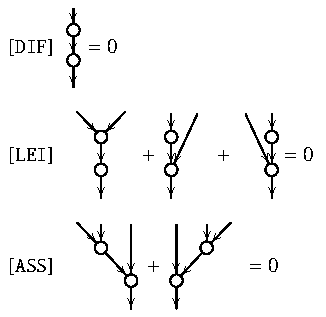
\includegraphics[width=0.32\paperwidth]{figures/Fig_013_PDF049_Book037.pdf}
  \caption{微分律、Leibniz 律与结合律的树形表示（原书 p.37）}
  \label{fig:basic-identity-trees}
\end{figure}
这种图示解释可以推广到所有 $k$。

\subsection{$A_\infty$ 代数}\label{subsec:ainfty-algebras}
\begin{definition}{$A_\infty$ 代数}{ainfty-algebra}
$A_\infty$ 代数\index{adaishu@$A_\infty$ 代数|hyperpage}是一个分次向量空间 $A^\bullet$，连同一列次数为 $1$ 的映射
\[
  b_i\colon A[1]^{\otimes i}\to A[1],\qquad i=1,2,\ldots,
\]
使得对所有 $n\geq1$ 都有恒等式
\[
  [M_n]\qquad
  \sum_{\substack{r+s+t=n\\r,t\geq0,\ s>0}}
  b_{r+t+1}\circ
  \bigl(1^{\otimes r}\otimes b_s\otimes1^{\otimes t}\bigr)=0.
\]
\end{definition}
上述公式可以图示为
\begin{figure}[H]\centering
  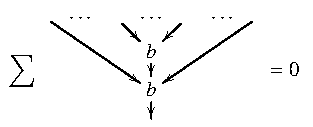
\includegraphics[width=0.37\paperwidth]{figures/Fig_014_PDF049_Book037.pdf}
  \caption{$A_\infty$ 代数恒等式的两节点树形表示（原书 p.37）}
  \label{fig:ainfty-algebra-trees}
\end{figure}
其中求和遍历所有具有 $n$ 个叶子、两个节点的根树。

\begin{note}
次数为 $1$ 的映射 $b_i\colon A[1]^{\otimes i}\to A[1]$，也可以看作次数为 $2-i$ 的映射
\[
  \mu_i\colon A^{\otimes i}\to A.
\]
从这个角度看，一元乘积的次数为 $1$，二元乘积的次数为 $0$，分别与微分和通常的乘积相同。这一次数约定也符合三元 Massey 积
\[
  \langle u,v,w\rangle
  =\bigl[u\,d^{-1}(vw)\pm d^{-1}(uv)\,w\bigr]
\]
的定义；三元 Massey 积的次数是 $-1=2-3$。此外，定理\ref{thm:ext-low-degrees}之后的讨论表明，高阶乘积应当记录关系的系数
\[
  \mu_k(\xi_1\otimes\cdots\otimes\xi_k)=\sum_i\lambda_i\rho_i,
\]
其中 $\xi_i\in\operatorname{Ext}_A^1(S,S)$，$\rho_i\in\operatorname{Ext}_A^2(S,S)$。因此，这里的次数同样为
\[
  \deg\rho_i-\deg\xi_1-\cdots-\deg\xi_k=2-k.
\]
\end{note}

\begin{note}
条件 $[M_1]$ 与 $[\mathrm{DIF}]$ 相同，因此 $(A[1],b_1)$ 总是一个上链复形。条件 $[M_2]$ 与 $[\mathrm{LEI}]$ 相同；若 $b_1=0$ 或 $b_3=0$，条件 $[M_3]$ 就化为 $[\mathrm{ASS}]$，因为其余各项都同时含有 $b_1$ 和 $b_3$。
\end{note}

\subsection{$A_\infty$ 态射}\label{subsec:ainfty-morphisms}
自然地，我们也希望定义 $A_\infty$ 代数之间的态射\index{ataishe@$A_\infty$ 态射|hyperpage}。直观上，人们可能会认为态射就是满足
\[
  b_k^B\circ f^{\otimes k}=f\circ b_k^A
\]
的映射 $f\colon A\to B$。遗憾的是，这个概念过于严格，因为它不允许不同乘积相互混合。它只能把 $A$ 的 $k$ 元乘积与 $B$ 的 $k$ 元乘积联系起来；但我们引入高阶乘积，正是为了在取同调时保留二元乘积的一些特征。因此，需要一种允许不同乘积相互混合的态射概念。

\begin{definition}{$A_\infty$ 态射}{ainfty-morphism}
$A_\infty$ 态射 $f_\bullet\colon A\to B$ 是一列次数为 $0$ 的映射
\[
  f_i\colon A[1]^{\otimes i}\to B[1],
\]
并满足以下公理：
\[
  [F_n]\qquad
  \sum_{\substack{r+s+t=n\\r,t\geq0,\ s>0}}
  f_{r+t+1}\circ
  \bigl(1^{\otimes r}\otimes b_s^A\otimes1^{\otimes t}\bigr)
  =
  \sum_{\substack{i_1+\cdots+i_k=n\\k>0,\ i_j>0}}
  b_k^B\circ(f_{i_1}\otimes\cdots\otimes f_{i_k}).
\]
两个 $A_\infty$ 态射 $f_\bullet\colon A\to B$ 和 $g_\bullet\colon B\to C$ 的复合定义为
\[
  (g\circ f)_n:=
  \sum_{\substack{i_1+\cdots+i_k=n\\k>0,\ i_j>0}}
  g_k\circ(f_{i_1}\otimes\cdots\otimes f_{i_k}).
\]
$[F_1]$ 表明，$f_1$ 是上链复形 $(A[1],b_1^A)$ 与 $(B[1],b_1^B)$ 之间的态射。若 $f_1$ 是上链复形同构\index{atonggou@$A_\infty$ 同构|hyperpage}，则称 $f_\bullet$ 为 $A_\infty$ 同构；若 $f_1$ 是拟同构\index{anitonggou@$A_\infty$ 拟同构|hyperpage}，则称 $f_\bullet$ 为 $A_\infty$ 拟同构。
\end{definition}

\begin{note}
$A_\infty$ 态射公理可以图示如下：
\begin{figure}[H]\centering
  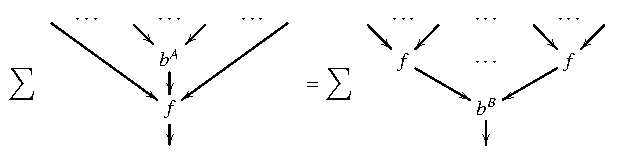
\includegraphics[width=0.77\paperwidth]{figures/Fig_015_PDF051_Book039.pdf}
  \caption{$A_\infty$ 态射公理的图示（原书 p.39）}
  \label{fig:ainfty-morphism-diagram}
\end{figure}
若所有高阶映射都为零（$f_{\geq2}=0$），就恢复了朴素的态射定义。这类态射称为严格 $A_\infty$ 态射。若 $g_\bullet\colon B^\bullet\to A^\bullet$ 是 $f_\bullet\colon A^\bullet\to B^\bullet$ 的（拟）逆，则要求它们的复合为严格态射，且 $g_1$ 是 $f_1$ 的（拟）逆。于是 $(f\circ g)_1$ 和 $(g\circ f)_1$ 分别（同伦于）恒等映射。
\end{note}

\begin{lemma}{$A_\infty$ 态射的逆}{ainfty-morphism-inverse}
设 $f_\bullet\colon A^\bullet\to B^\bullet$ 是一个 $A_\infty$ 态射。
\begin{enumerate}
  \item $f_\bullet$ 有逆，当且仅当它是 $A_\infty$ 同构；
  \item $f_\bullet$ 有拟逆，当且仅当它是 $A_\infty$ 拟同构。
\end{enumerate}
\end{lemma}
\begin{proof}[证明思路]
思路是逐步构造（拟）逆 $g_\bullet$。先构造 $g_1$：由于 $f_1$ 是（拟）同构，由引理\ref{lem:complex-map-criterion}可取其（拟）逆 $g_1$。更高阶的 $g_i$ 可由条件 $(g\circ f)_{>0}=0$ 归纳确定。例如，若 $g_1$ 是同构且 $(g\circ f)_2=0$，则
\[
  g_2(f_1\otimes f_1)+g_1f_2=0,
\]
因此
\[
  g_2=-g_1f_2(f_1^{-1}\otimes f_1^{-1})
      =-g_1f_2(g_1\otimes g_1).
\]
另见\bookcite[I 1.14]{218}。
\end{proof}

与复形态射一样，$A_\infty$ 态射的强大之处在于拟同构可以取拟逆。若只允许严格态射，这一点便不再成立。严格态射的拟逆一般不再严格，因为要使它满足公理 $[F_n]$，通常需要非零的高阶分量。

\subsection{处理符号}\label{subsec:sign-conventions}
若工作域的特征为 $0$，乘积 $b_2$ 并不给出通常意义下的乘积，因为结合律只在相差符号的意义下成立。因此，需要额外引入符号才能使各项协调一致。处理这一问题有多种方法；简要综述可参见\bookcite{202}。

起点是 Koszul 符号约定，它规定如何让算子作用于输入元。

\begin{definition}{Koszul 符号约定}{koszul-sign}
设 $\varphi\colon V^{\otimes k}\to V$、$\psi\colon V^{\otimes l}\to V$ 是两个分次线性算子。定义它们的张量积在 $V^{\otimes(k+l)}$ 上的左作用为
\[
  (\varphi\otimes\psi)
  (a_1\otimes\cdots\otimes a_k\otimes b_1\otimes\cdots\otimes b_l)
  =
  (-1)^{|\psi|(|a_1|+\cdots+|a_k|)}
  \varphi(a_1\otimes\cdots\otimes a_k)
  \otimes
  \psi(b_1\otimes\cdots\otimes b_l),
\]
其中 $|a|$ 简记元素 $a$ 的次数。
\end{definition}
换言之，Koszul 规则是：每当一个奇次数算子越过一个奇次数元素时，就要引入一个负号。这个经验法则也能给出算子从右侧作用时的公式：
\[
  (a_1\otimes\cdots\otimes a_k\otimes b_1\otimes\cdots\otimes b_l)
  (\varphi\otimes\psi)
  =
  (-1)^{|\varphi|(|b_1|+\cdots+|b_l|)}
  \varphi(a_1\otimes\cdots\otimes a_k)
  \otimes\psi(b_1\otimes\cdots\otimes b_l).
\]
从这里开始，有两种主要的符号约定：一种主要用于辛几何，另一种主要用于表示论。

\subsubsection*{辛几何约定}
Seidel 的著作\bookcite{218}与大多数关于 Fukaya 范畴的论文都采用这种约定。令移位后的乘积 $b_\bullet$ 和 $A_\infty$ 态射 $f_\bullet$ 从右侧作用，并定义
\[
  \mu_k(a_1,\ldots,a_k)
  :=\bigl((a_1[1]\otimes\cdots\otimes a_k[1])b_k\bigr)[-1],
\]
\[
  \varphi_k(a_1,\ldots,a_k)
  :=\bigl((a_1[1]\otimes\cdots\otimes a_k[1])f_k\bigr)[-1],
\]
其中 $a[1]$ 表示把 $a\in A$ 看作 $A[1]$ 中的元素；在 $A[1]$ 中它的次数降低 $1$。由此得到以下版本的 $A_\infty$ 公理：
\[
  [\mathrm{SM}_n]\qquad
  \sum_{r+s+t=n}(-1)^\dagger
  \mu_{r+t+1}(a_1,\ldots,a_r,\mu_s(a_{r+1},\ldots,a_{r+s}),
       a_{r+s+1},\ldots,a_{r+s+t})=0,
\]
其中
\[
  \dagger=(|a_{r+s+1}|-1)+\cdots+(|a_{r+s+t}|-1).
\]
指数中出现 $|a_{r+s+1}|-1$，是因为输入元素的次数已经移位。
% [Tutor Note: 这里 $|\cdot|$ 是元素在 $A$ 中的次数，不是移位后在 $A[1]$ 中的次数，所以每越过一个输入就贡献 $(|a|-1)$；若误把输入当成 $A[1]$ 的元素（次数 $|a|-1$）再算，会多出符号。另一处常见混淆是 $\mu$ 与 $m$ 两套约定：$m_k=\sigma^{-1}\circ b_k\circ\sigma^{\otimes k}$ 不带额外符号，而 $\mu$ 由右作用 $\bigl((a_1[1]\otimes\cdots\otimes a_k[1])b_k\bigr)[-1]$ 定出，两者只差整体符号约定，切勿混用。]

若 $A_\infty$ 代数满足 $\mu_{\geq3}=0$，则规则 $[\mathrm{SM}_2]$ 与 $[\mathrm{SM}_3]$ 分别化为
\[
  \mu_1(\mu_2(a,b))
  +(-1)^{|b|-1}\mu_2(\mu_1(a),b)
  +\mu_2(a,\mu_1(b))=0,
\]
\[
  (-1)^{|c|-1}\mu_2(\mu_2(a,b),c)
  +\mu_2(a,\mu_2(b,c))=0.
\]
遗憾的是，这两式都不是通常的 Leibniz 律或结合律。可以通过另外定义
\[
  da:=(-1)^{|a|}\mu_1(a),
  \qquad
  a\cdot b:=(-1)^{|b|}\mu_2(a,b)
\]
来解决。于是有
\begin{align*}
  &(-1)^{|a|+|b|+|b|}d(a\cdot b)
  +(-1)^{|b|-1+|a|+|b|}da\cdot b
  +(-1)^{|b|+|b|+1}a\cdot db=0,\\
  &(-1)^{|a|}\bigl(d(a\cdot b)-da\cdot b-(-1)^{|a|}a\cdot db\bigr)=0,\\
  &(-1)^{|c|-1+|b|+|c|}(a\cdot b)\cdot c
  +(-1)^{|b|+|c|+|c|}a\cdot(b\cdot c)=0,\\
  &(-1)^{|b|-1}\bigl((a\cdot b)\cdot c-a\cdot(b\cdot c)\bigr)=0.
\end{align*}
对 $A_\infty$ 态射，相应的符号规则为
\[
  [\mathrm{SF}_n]\qquad
  \sum_{\substack{r+s+t=n\\r,t\geq0,\ s>0}}(-1)^\dagger
  \varphi_{r+t+1}\circ
  (1^{\otimes r}\otimes\mu_s^A\otimes1^{\otimes t})
  =
  \sum_{\substack{i_1+\cdots+i_k=n\\k>0,\ i_j>0}}
  \mu_k^B\circ(\varphi_{i_1}\otimes\cdots\otimes\varphi_{i_k}).
\]
注意，$\varphi$ 前面没有额外符号，因为它们的移位版本次数为 $0$。

\subsubsection*{表示论约定}
Keller 的综述文章\bookcite{133}、\bookcite{135}与许多高阶代数论文采用这种约定。先定义次数为 $-1$ 的映射
\[
  \sigma\colon A\to A[1],\qquad x\longmapsto(-1)^{|x|}x[1].
\]
令移位后的乘积 $b_\bullet$ 和 $A_\infty$ 态射 $f_\bullet$ 从左侧作用，并定义未移位乘积
\[
  m_k(a_1,\ldots,a_k)
  :=\sigma^{-1}\circ b_k\circ\sigma^{\otimes k}
       (a_1\otimes\cdots\otimes a_k).
\]
态射分量也按相同方式解除移位：若把移位后的分量记为 $f_k^{\mathrm{sh}}$，则令
\[
  f_k(a_1,\ldots,a_k)
  :=\sigma_B^{-1}\circ f_k^{\mathrm{sh}}\circ\sigma_A^{\otimes k}
       (a_1\otimes\cdots\otimes a_k).
\]
这样得到的 $A_\infty$ 公理为
\[
  [\mathrm{RM}_n]\qquad
  \sum_{r+s+t=n}(-1)^\epsilon
  m_{r+t+1}(a_1,\ldots,a_r,m_s(a_{r+1},\ldots,a_{r+s}),
      a_{r+s+1},\ldots,a_{r+s+t})=0,
\]
其中
\[
  \epsilon=r+st+s(|a_1|+\cdots+|a_r|).
\]
注意，在这种约定下，Leibniz 律和结合律会自动出现：
\begin{align*}
  &(-1)^{0+2\cdot0}m_1(m_2(a,b))
  +(-1)^{0+1\cdot1}m_2(m_1(a),b)
  +(-1)^{1+1\cdot0+|a|}m_2(a,m_1(b))=0,\\
  &(-1)^{0+2\cdot1}m_2(m_2(a,b),c)
  +(-1)^{1+2\cdot0+2|a|}m_2(a,m_2(b,c))=0.
\end{align*}

\begin{note}
我们始终用字母 $b$ 记移位后的映射，用拉丁字母 $m$ 记表示论约定，用希腊字母 $\mu$ 记辛几何约定。由于研究 Fukaya 范畴时后一种约定十分重要，下面大多采用 $\mu$-乘积，并以带有相应符号的 $\mu$-乘积表述定义。这些符号来自只含加号的 $b$-乘积定义。
\end{note}

\subsection{例子}\label{subsec:ainfty-examples}
\begin{example}[普通代数]\label{ex:ordinary-algebra-ainfty}
任意普通代数 $(R,\cdot)$ 都可以看成集中在次数 $0$ 的 $A_\infty$ 代数 $R^\bullet$，其中 $\mu_2(x,y)=x\cdot y$，且 $\mu_i=0$（$i\neq2$）。
\end{example}

\begin{example}[微分分次代数]\label{ex:dg-algebra-ainfty}
若 $(A,d,\cdot)$ 是 dg-代数，我们将其视为具有如下 $\mu$-乘积的 $A_\infty$ 代数：
\[
  da:=(-1)^{|a|}\mu_1(a),
  \qquad
  a\cdot b:=(-1)^{|b|}\mu_2(a,b).
\]
\end{example}

\begin{example}[dg-代数拟同构不必反向存在]\label{ex:dg-quasiisomorphism-ainfty}
考虑普通代数 $R=k[X]/(X^2)$ 和 dg-代数 $A=k[X,Y]/(Y^2)$，其中 $|X|=0$、$|Y|=-1$，且 $dY=X^2$。由于 $R^\bullet$ 是 $A^\bullet$ 的同调，存在 dg-代数拟同构 $\pi\colon A^\bullet\to R^\bullet$；它对应于一个严格的 $A_\infty$ 拟同构。

反方向不存在 dg-代数拟同构，因为 $X^2$ 在 $R$ 中为零，而 $A$ 的零次部分没有零因子。不过，我们可以构造一个 $A_\infty$ 拟同构 $\varphi_\bullet\colon R^\bullet\to A^\bullet$，令
\[
  \varphi_1(a+bX)=a+bX,\qquad
  \varphi_2(1,X)=\varphi_2(X,1)=0,\qquad
  \varphi_2(X,X)=Y.
\]
由次数考虑，所有更高阶的 $\varphi_i$ 都必须为零。对于 $(X,X)$，$A_\infty$ 规则 $[\mathrm{SF}_2]$ 变成
\[
  \varphi_1\mu_2^R(X,X)
  =\mu_2^A(\varphi_1(X),\varphi_1(X))
   +\mu_1^A(\varphi_2(X,X)),
\]
也就是
\[
  0=X^2+(-1)^{|Y|}dY=X^2-X^2.
\]
\end{example}

\begin{example}[形式幂级数与 $A_\infty$ 结构]\label{ex:ainfty-formal-series}
设 $r\in k[[X]]$ 是常数项为零的形式幂级数：
\[
  r=r_1X+r_2X^2+r_3X^3+\cdots.
\]
令 $A=k\xi\oplus k\rho$，其中 $|\xi|=1$、$|\rho|=2$。定义如下 $A_\infty$ 结构：
\[
  \mu_k^r(\xi,\ldots,\xi)=r_k\rho,
\]
而所有含有 $\rho$ 的乘积都规定为零。容易验证这些乘积满足 $A_\infty$ 公理。

再取另一个形式幂级数
\[
  f=f_1X+f_2X^2+\cdots\in k[[X]].
\]
它定义环同态
\[
  \iota_f\colon k[[X]]\to k[[X]],\qquad
  u(X)\longmapsto u(f(X)).
\]
令 $s=\iota_f(r)$。定义 $A_\infty$ 映射 $\varphi_k^f\colon A^{\otimes k}\to A$：
\[
  \varphi_k^f(\xi,\ldots,\xi)=f_k\xi.
\]
所有含有 $\rho$ 的表达式都映为零，只有 $\varphi_1^f(\rho)=\rho$ 例外。于是得到从 $(A,\mu^s)$ 到 $(A,\mu^r)$ 的 $A_\infty$ 态射。其关键恒等式为
\begin{align*}
  &\mu_k^r\bigl(\varphi_{i_1}^f(\xi,\ldots,\xi),\ldots,
                       \varphi_{i_k}^f(\xi,\ldots,\xi)\bigr)\\
  &\quad=\sum_{i_1+\cdots+i_k=n}
       \mu_k^r(f_{i_1}\xi,\ldots,f_{i_k}\xi)
   =\sum_{i_1+\cdots+i_k=n}f_{i_1}\cdots f_{i_k}r_k\rho\\
  &\quad=\varphi_1^f\mu_n^s(\xi,\ldots,\xi)
   =\sum_{i+j+k=n}
     \varphi^f(\ldots,\mu_j^s(\xi,\ldots,\xi),\ldots).
\end{align*}
两个这样的 $A_\infty$ 态射的复合，对应于 $k[[X]]$ 上两个环同态的复合：
\[
  \varphi_\bullet^f\circ\varphi_\bullet^g=\varphi_\bullet^h,
  \qquad \iota_f\circ\iota_g=\iota_h.
\]
最后，若 $f_1\neq0$，则 $\iota_f$ 可逆，因此 $\varphi_\bullet^f$ 是 $A_\infty$ 同构。从某种意义上说，$A$ 上的 $A_\infty$ 结构与 $k[[X]]$ 中的元素互为对偶。
\end{example}

\begin{note}
还可以在前一个例子中加入一个次数为 $0$ 的单位元：
\[
  E^\bullet=k1\oplus k\xi\oplus k\rho.
\]
对乘积增加如下规则：对任意齐次元 $u\in E^\bullet$，
\[
  \mu_2^r(u,1)=(-1)^{|u|}\mu_2^r(1,u)=u;
\]
而所有其他含有 $1$ 的乘积均规定为零。
\end{note}

\section{极小模型}\label{sec:minimal-models}
\takeaway{用复形分裂定理把 $A_\infty$ 代数拆成可缩部分与极小部分的直和；极小模型由对树求和定义，故在 $A_\infty$ 同构意义下唯一；同调扰动引理把这套树形公式推广到任意拟同构，是 dg-模型与极小模型互转的工具。}
\subsection{结构定理}\label{subsec:ainfty-structure-theorem}
与向量空间复形类似，$A_\infty$ 代数也有一个结构定理，它允许我们把每个 $A_\infty$ 代数分解为两部分的直和。

\begin{definition}{极小与可缩的 $A_\infty$ 结构}{minimal-contractible-ainfty}
$A_\infty$ 结构 $(A,b)$ 称为
\begin{itemize}
  \item 极小的，若 $b_1=0$；
  \item 可缩的，若 $b_{>1}=0$ 且 $H(A)=0$。
\end{itemize}
\end{definition}

\begin{theorem}{Kadeishvili 极小模型定理}{kadeishvili-minimal-model}
每个 $A_\infty$ 代数都 $A_\infty$ 同构于一个可缩 $A_\infty$ 代数\index{kesuoadaishu@可缩 $A_\infty$ 代数|hyperpage}与一个极小 $A_\infty$ 代数\index{jixiaoadaishu@极小 $A_\infty$ 代数|hyperpage}的直和\bookcite{131}。
\end{theorem}
\begin{proof}[证明思路]
这里概述 Kontsevich 与 Soibelman 的证明\bookcite{147}，因为它有很好的图示解释。Merkulov 和 Markl 的其他较详细论述见\bookcite{174}、\bookcite{170}。

设 $A$ 是一个 $A_\infty$ 代数。对 $A$ 上的微分 $-b_1$，按照引理\ref{lem:complex-map-criterion}选取分解
\[
  A^\bullet=I^\bullet\oplus H^\bullet\oplus R^\bullet.
\]
这给出一个映射 $h$ 与投影
\[
  \pi=1+b_1h+hb_1,
\]
其像为 $H^\bullet$。
\begin{figure}[H]\centering
  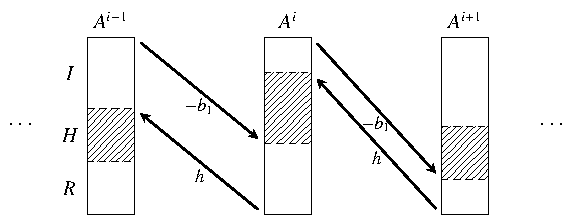
\includegraphics[width=0.46\paperwidth]{figures/Fig_016_PDF055_Book043.pdf}
  \caption{上链复形 $(A,b_1)$ 的极小与可缩部分（原书 p.43）}
  \label{fig:ainfty-minimal-splitting}
\end{figure}
上链复形 $(A,b_1)$ 分解为 $A_{\mathrm{contr}}\oplus A_{\min}$，其中
\[
  A_{\mathrm{contr}}=I^\bullet\oplus R^\bullet=\ker\pi,
  \qquad
  A_{\min}=H^\bullet=\operatorname{im}\pi.
\]
\end{proof}

新结构 $\bar b$ 应当与上述分解相容，并且要构造 $(A,b)$ 与 $(A,\bar b)$ 之间的 $A_\infty$ 同构 $f_\bullet$。我们保留一元乘积不变，即 $\bar b_1=b_1$。要计算更高阶的 $\bar b_k$，考察具有 $k$ 个叶子的树。对每一棵这样的树 $T$，都可以构造一个乘积 $b_T$：每个叶子表示映射 $\pi$，每个节点表示某个映射 $b_i$，每条内部边表示映射 $h$，而树干表示 $\pi$。

\begin{figure}[H]\centering
  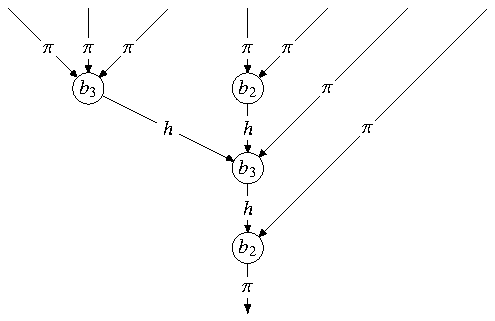
\includegraphics[width=0.43\paperwidth]{figures/Fig_017_PDF056_Book044.pdf}
  \caption{由树构造高阶乘积的示意图（原书 p.44）}
  \label{fig:tree-higher-products}
\end{figure}
上图对应的乘积为
\[
  b_T=\pi b_2\bigl(hb_3(hb_3\pi^{\otimes3}\otimes hb_2\pi^{\otimes2}\otimes\pi)\otimes\pi\bigr).
\]
定义新乘积为所有这些 $b_T$ 之和：
\[
  \bar b_k:=\sum_T b_T.
\]
% [Tutor Note: 书中只说“每个节点表示某个映射 $b_i$”，未限定 $i\geq2$。若允许 $b_1$ 作节点标记，$k$ 个叶子的树可以带任意长的 $b_1$ 单链，$\bar b_k$ 的定义就不再是有限和（形式的 $\partial_h$ 也需要幂级数收敛性才能逐项求导）。标准约定只取 $i\geq2$：每个内节点至少 $2$ 个儿子，故含 $k$ 个叶子的树至多 $k-1$ 个内节点，求和确为有限和。]
由于 $b_T$ 中都含有 $\pi$，新高阶乘积 $\bar b_\bullet$ 的像落在 $A_{\min}$ 中；只要某个输入属于 $A_{\mathrm{contr}}$，它就为零。另一方面，$\bar b_1$ 的像落在 $A_{\mathrm{contr}}$ 中，并且在 $A_{\min}$ 上为零。因此
\[
  (A,\bar b)=(A_{\mathrm{contr}},\bar b_1)\oplus(A_{\min},\bar b_{>1}).
\]

为证明 $\bar b$ 满足 $A_\infty$ 关系，注意算子 $\bar b_k$ 依赖于 $h$，可以对其求偏导：
\[
  \partial_h\bar b_k[u]
  :=\lim_{\varepsilon\to0}
  \frac{\bar b_k^{h+\varepsilon u}-\bar b_k^h}{\varepsilon}.
\]
这个导数等于把每棵树中的一条 $h$ 替换成 $u$ 后所得各项之和。若令 $u=\pi^2$，并沿这两个 $\pi$ 之间的边把树切开，就得到两棵较小的树。因此
\[
  \partial_h\bar b_k[\pi^2]
  =\sum_T\sum_{\substack{\text{树 }T\text{ 中}\\\text{的一条边 }h}}b_T
  =\sum_{T_1,T_2}
    b_{T_1}(\cdots\otimes b_{T_2}\otimes\cdots).
\]
表达式 $\partial_h\bar b_k[\pi^2]$ 实际上组合了所有成对出现的高阶乘积 $\bar b_{\geq2}$。这几乎就是 $\bar b$ 的 $A_\infty$ 关系，除了含有 $\bar b_1$ 的项。幸运的是，所有一个因子为 $\bar b_1$、另一个因子为 $\bar b_{\geq2}$ 的项都为零，因为 $b_1\pi=\pi b_1=0$。因此，$\bar b$ 的 $A_\infty$ 关系 $[M_k]$ 可以写成
\[
  \partial_h\bar b_k[\pi^2]=0.
\]
代入
\[
  \pi^2=\pi=1+b_1h+hb_1
\]
后，有
\[
  \partial_h\bar b_k[\pi^2]
  =\partial_h\bar b_k[1]
   +\partial_h\bar b_k[b_1h]
   +\partial_h\bar b_k[hb_1].
\]
最后两项是对所有树和边求和，其中 $b_1$ 被插在该边之前或之后。和中的每一项都含有 $b_l(\cdots b_1\cdots)$ 或 $b_1b_l$，其中 $l\geq2$。利用 $b$ 的 $A_\infty$ 关系，可将这些项改写成所有 $b_r(\cdots b_s\cdots)$ 的负和，其中 $r,s\geq2$。这样的乘积将 $b_r$ 与 $b_s$ 直接相连，中间没有 $h$，所以得到的都是把一条 $h$ 替换成 $1$ 的树。因此
\[
  \partial_h\bar b_k[b_1h]+\partial_h\bar b_k[hb_1]
  =-\partial_h\bar b_k[1],
\]
从而 $\partial_h\bar b_k[\pi^2]=0$，故 $\bar b$ 满足 $A_\infty$ 公理。

证明 $(A,b)$ 与 $(A,\bar b)$ 之间存在满足 $f_1=1$ 的 $A_\infty$ 同构 $f_\bullet$，只需进行类似计算。$f_i$ 的公式与 $\bar b_i$ 相同，只是树根处用映射 $h$ 代替 $\pi$。

\begin{note}
注意，对序列 $a_1\otimes\cdots\otimes a_n$ 使用 $\bar b$ 的公式时，不会出现来自 Koszul 规则的额外符号，因为所有涉及的映射（$\pi$ 和 $h\circ b$）次数都是偶数。因此，该公式对 $\mu$-乘积也成立，无须额外加入符号。

由于 $(A,\bar b)$ 是直和，嵌入 $A_{\min}\hookrightarrow A$ 和投影 $A\to A_{\min}$ 都是严格态射。

将嵌入与 $f_\bullet$ 的逆 $f_\bullet^{-1}\colon(A,\bar b)\to(A,b)$ 复合，并将投影与 $f_\bullet\colon(A,b)\to(A,\bar b)$ 复合，就得到映射
\[
  i_\bullet\colon A_{\min}\to(A,b),\qquad
  p_\bullet\colon(A,b)\to A_{\min}.
\]
若 $g_\bullet\colon A^\bullet\to B^\bullet$ 是 $A_\infty$ 拟同构，则
\[
  p_\bullet^B\circ g_\bullet\circ i_\bullet^A
\]
是两个极小模型之间的 $A_\infty$ 同构。反过来，若 $g_\bullet\colon A_{\min}^\bullet\to B_{\min}^\bullet$ 是 $A^\bullet,B^\bullet$ 的极小模型之间的 $A_\infty$ 同构，则
\[
  i_\bullet^B\circ g_\bullet\circ p_\bullet^A
\]
是 $A^\bullet$ 与 $B^\bullet$ 之间的 $A_\infty$ 拟同构。
\end{note}

\begin{corollary}{极小模型刻画拟同构}{minimal-models-characterize-quasi-isomorphism}
两个 $A_\infty$ 代数 $A_\infty$ 拟同构，当且仅当它们的极小模型 $A_\infty$ 同构。
\end{corollary}

自然的想法是构造 $A_\infty$ 代数的极小模型，并只研究极小模型，因为它们在 $A_\infty$ 同构意义下唯一确定。然而，实际算出极小模型的所有乘积出了名地困难；给定两个极小模型，要检验它们是否 $A_\infty$ 同构也很困难。

在另一端，也可以构造 dg-模型。它们是没有高阶乘积的 $A_\infty$ 代数，即 $b_{\geq3}=0$。dg-模型的优点是代数结构较容易处理，缺点则是含有许多在取同调时会被删去的额外元素。

具体应用不同，dg-模型或极小模型可能各有优势。$A_\infty$ 形式体系提供了一个框架，使我们能够相对容易地在不同模型之间转换。这可以借助同调扰动引理\index{tongdiaoraodongyinli@同调扰动引理|hyperpage}完成；它是极小模型定理的推广。

\begin{lemma}{同调扰动引理}{homological-perturbation-lemma}
设 $\varphi\colon A\to B$ 和 $\varphi^\dagger\colon B\to A$ 是两个复形 $(A,\mu_1^A)$、$(B,\mu_1^B)$ 之间互为拟逆的映射，并取映射 $h\colon B\to B$，满足
\[
  \varphi\varphi^\dagger=1_B+h\mu_1^B+\mu_1^Bh.
\]
\begin{figure}[H]\centering
  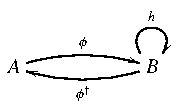
\includegraphics[width=0.35\paperwidth]{figures/Fig_018_PDF058_Book046.pdf}
  \caption{同调扰动引理中的链映射与同伦（原书 p.46）}
  \label{fig:homological-perturbation}
\end{figure}
若 $\mu_B^\bullet$ 是 $B$ 上延拓 $\mu_1^B$ 的一个 $A_\infty$ 结构，则可以把 $\mu_1^A$ 延拓为 $A_\infty$ 结构 $\mu_A^\bullet$，并构造 $A_\infty$ 拟同构 $\varphi_\bullet\colon A\to B$，使得 $\varphi_1=\varphi$。
\end{lemma}
\begin{proof}[证明思路]
思路相同：$\mu_n^A$ 是对所有树求和得到的，树节点标记为 $\mu_B$，叶子处是 $\varphi$，树根处是 $\varphi^\dagger$，内部边上是 $h$；构造 $\varphi_\bullet$ 时也用相同方法，只把树根处的映射换成 $h$。递归地，可以写为
\begin{align*}
  \mu_n^A(a_1,\ldots,a_n)
  &=
  \sum_r\ \sum_{\substack{i_1+\cdots+i_r=n\\i_j>0}}
  \varphi^\dagger\mu_r^B\bigl(
  \varphi_{i_1}(a_1,\ldots,a_{i_1}),\ldots,
  \varphi_{i_r}(a_{n-i_r+1},\ldots,a_n)\bigr),\\
  \varphi_n(a_1,\ldots,a_n)
  &=
  \sum_r\ \sum_{\substack{i_1+\cdots+i_r=n\\i_j>0}}
  h\mu_r^B\bigl(
  \varphi_{i_1}(a_1,\ldots,a_{i_1}),\ldots,
  \varphi_{i_r}(a_{n-i_r+1},\ldots,a_n)\bigr).
\end{align*}
更多细节见\bookcite{170}。
% [Tutor Note: 这两式都略去了下标与求和限制。$\mu_n^A$ 的式子右端用 $b$ 的 $\mu_r^B$ 与输入端的 $\varphi$，此时 $\varphi$ 已由下式先构造好，故 $r=1,\ i_1=n$ 也可；但 $\varphi_n$ 的递推必须取 $r\geq2$（即每个 $\varphi_{i_j}$ 的下标 $i_j\leq n-1$），否则右端会出现 $\mu_1^B\varphi_n$ 自身造成循环。书中把两式写成同一形式，读者需自行补上这一限制。]
\end{proof}

\subsection{例子}\label{subsec:minimal-model-examples}
\begin{example}[多项式环的 Ext 代数极小模型]\label{ex:minimal-model-polynomial}
回到例\ref{ex:ext-polynomial-two-variables}中的多项式环 $R=k[X,Y]$ 与 $S=R/(X,Y)$。我们已经知道
\[
  \operatorname{Ext}_R^\bullet(S,S)
  =\frac{k\langle\xi,\eta\rangle}
  {\langle\xi^2,\eta^2,\xi\eta+\eta\xi\rangle}.
\]
这个计算是通过考察 $\operatorname{Hom}_R^\bullet(K^\bullet,K^\bullet)$ 的上同调得到的，其中
\[
  K^\bullet:=R\xrightarrow{\binom{X}{-Y}}R^2
  \xrightarrow{(X\ \ Y)}R.
\]

除了上同调分次外，还可以给 $K^\bullet$ 加上第二种分次：把 $R$ 看成 $X,Y$ 次数均为 $1$ 的分次环。就这个第二分次而言，$\iota,\xi,\eta,\rho$ 的次数都是 $0$，因为例\ref{ex:ext-polynomial-two-variables}中的计算表明，这些映射只含常数。微分 $b_1$ 的第二次数为 $1$，因为它关于 $X,Y$ 是线性的。如果选取与新分次相容的分解 $H\oplus I\oplus R$，则 $h$ 的次数为 $-1$。

构造高阶乘积时需要对所有树求和。树的每个节点都是普通乘积，故其第二次数为 $0$；每条内部边的第二次数为 $-1$，因为它表示 $h$。因此，所有高阶乘积的第二次数都为负数。由于 $\operatorname{Ext}_R^\bullet(S,S)$ 只含第二次数为 $0$ 的元素，可以得出所有高阶乘积均为零。
\end{example}

\begin{example}[非零三元乘积]\label{ex:nonzero-triple-product}
考察
\[
  A=\frac{k\langle X,Y\rangle}{\langle X^2Y\rangle},
\]
并令 $S=A/(X,Y)$ 为 $X,Y$ 均平凡作用的简单右模。该模的 Koszul 分解为
\[
  K^\bullet:=A\xrightarrow{\binom{XY}{0}}A^{\oplus2}
  \xrightarrow{(X\ \ Y)}A.
\]
其 Ext 代数为
\[
  \operatorname{Ext}_A^\bullet(S,S)
  =k\iota\oplus(k\xi\oplus k\eta)\oplus k\rho.
\]
我们可以将这四个生成元提升为复形态射：
\begin{figure}[H]\centering
  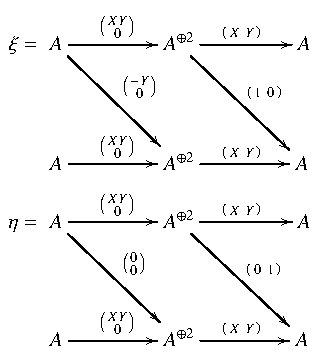
\includegraphics[width=0.48\paperwidth]{figures/Fig_019_PDF059_Book047.pdf}
  \caption{Ext 代数生成元 $\xi,\eta$ 的复形态射提升（原书 p.47）}
  \label{fig:nonzero-massey-generators}
\end{figure}
从这些表达式可知
\[
  \eta\cdot\xi=\eta\cdot\eta=\xi\cdot\eta=0,
\]
而 $\xi\cdot\xi$ 可由下图表示：
\begin{figure}[H]\centering
  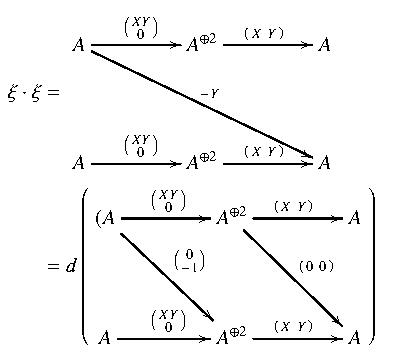
\includegraphics[width=0.46\paperwidth]{figures/Fig_020_PDF060_Book048.pdf}
  \caption{$\xi\cdot\xi$ 在 Hom 复形中为边界（原书 p.48）}
  \label{fig:xi-square-boundary}
\end{figure}
因此，尽管 $\xi\cdot\xi$ 在 $\operatorname{Hom}_A^\bullet(S,S)$ 中非零，它在上同调中为零：$\xi\cdot\xi=d\kappa$。由于 $\xi,\kappa$ 的次数均为 $1$，这一恒等式写成
\[
  -\mu_2(\xi,\xi)=-\mu_1(\kappa).
\]
在 $\operatorname{Hom}_A^\bullet(K^\bullet,K^\bullet)$ 中选取分解 $R\oplus H\oplus I$，其基包含 $\iota,\xi,\eta,\rho\in H$、$\xi\cdot\xi\in I$ 和 $\kappa\in R$。于是
\[
  h\mu_2(\xi,\xi)=-\kappa.
\]
计算 $\bar\mu_3$ 时，需要对下列两棵树求和：
\begin{figure}[H]\centering
  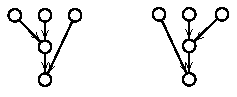
\includegraphics[width=0.29\paperwidth]{figures/Fig_021_PDF060_Book048.pdf}
  \caption{三元高阶乘积对应的两棵树（原书 p.48）}
  \label{fig:triple-product-trees}
\end{figure}
由此得到三元乘积
\begin{align*}
  \bar\mu_3(\eta,\xi,\xi)
  &=\pi\bigl(\mu_2(h\mu_2(\eta,\xi),\xi)
            +\mu_2(\eta,h\mu_2(\xi,\xi))\bigr)\\
  &=\pi(0-\mu_2(\eta,\kappa))
   =\pi(\eta\cdot\kappa)=-\rho,
\end{align*}
它非零。另一方面，
\begin{align*}
  \bar\mu_3(\xi,\xi,\eta)
  &=\pi\bigl(\mu_2(h\mu_2(\xi,\xi),\eta)
            +\mu_2(\xi,h\mu_2(\xi,\eta))\bigr)\\
  &=\pi(-\mu_2(\kappa,\xi)-0)
   =\pi(\kappa\cdot\xi)=0.
\end{align*}
这个例子可以推广为以下定理。
\end{example}

\begin{theorem}{Lu、Palmieri、Wu、Zhang 定理}{lu-palmieri-wu-zhang}
见\bookcite{168}。设
\[
  A=\frac{k\langle X_1,\ldots,X_n\rangle}
  {\langle r_1,\ldots,r_m\rangle}
\]
是一个极小表现，$S=A/\langle X_1,\ldots,X_n\rangle$ 是相应的简单模。$\operatorname{Ext}_A^\bullet(S,S)$ 的极小模型满足：
\begin{enumerate}
  \item $\operatorname{Ext}_A^1(S,S)=k\xi_1\oplus\cdots\oplus k\xi_n$；
  \item $\operatorname{Ext}_A^2(S,S)=k\rho_1\oplus\cdots\oplus k\rho_m$；
  \item 若关系 $r_j$ 中 $X_{i_k}\cdots X_{i_1}$ 的系数为 $\lambda_j$，则
  \[
    \mu(\xi_{i_1},\ldots,\xi_{i_k})
    =\sum_j\pm\lambda_j\rho_j.
  \]
\end{enumerate}
\end{theorem}

\begin{note}
符号和单项式的次序取决于具体采用的符号约定，也取决于所用的是右模（顺序反转）还是左模（保持原顺序）。
\end{note}

\section{\texorpdfstring{$A_\infty$}{A-infinity} 范畴}\label{sec:ainfty-categories}
\takeaway{$A_\infty$ 范畴的 $n$ 元乘积次数为 $2-n$；扭曲复形由满足 Maurer--Cartan 方程的次数 $1$ 元素 $\delta$ 给出，扭曲乘积在输入之间插入 $\delta$；取扭曲完备化的极小模型即得导出 $A_\infty$ 范畴，锥构造产生新对象，生成元生成整个导出范畴。}
\subsection{从代数到范畴}\label{subsec:algebras-to-categories}
正如 $k$-线性范畴可以看成代数的推广，也可以定义 $A_\infty$ 范畴。

\begin{definition}{$A_\infty$ 范畴与函子}{ainfty-category-functor}
$A_\infty$ 范畴\index{afanchou@$A_\infty$ 范畴|hyperpage} $\mathcal C^\bullet$ 由一族对象 $\operatorname{Ob}\mathcal C^\bullet$、分次 $k$-向量空间 $\mathcal C^\bullet(A,B)$ 与乘积构成：
\[
  \mu_n\colon
  \mathcal C^\bullet(A_1,A_0)\otimes\cdots\otimes
  \mathcal C^\bullet(A_n,A_{n-1})
  \longrightarrow\mathcal C^\bullet(A_n,A_0).
\]
这些乘积的次数为 $2-n$，并在所有有定义的地方满足带符号的广义结合律 $[\mathrm{SM}_n]$。

$A_\infty$ 函子\index{ahanzi@$A_\infty$ 函子|hyperpage} $F\colon\mathcal A^\bullet\to\mathcal B^\bullet$ 由对象映射
\[
  F\colon\operatorname{Ob}\mathcal A^\bullet\to
  \operatorname{Ob}\mathcal B^\bullet
\]
与映射
\[
  F_n\colon
  \mathcal A^\bullet(A_1,A_0)\otimes\cdots\otimes
  \mathcal A^\bullet(A_n,A_{n-1})
  \longrightarrow\mathcal B^\bullet(FA_n,FA_0)
\]
组成。$F_n$ 的次数为 $1-n$，并在所有有定义的地方满足带符号的广义结合律 $[\mathrm{SF}_n]$。$A_\infty$ 函子的复合与 $A_\infty$ 态射的复合定义相同。
\end{definition}

给定 $A_\infty$ 范畴 $\mathcal C^\bullet$，同样可以定义其极小模型，记为 $H\mathcal C^\bullet$；相应的嵌入和投影 $A_\infty$ 函子记作
\[
  I\colon H\mathcal C^\bullet\to\mathcal C^\bullet,\qquad
  P\colon\mathcal C^\bullet\to H\mathcal C^\bullet.
\]

\begin{note}
构造 $A_\infty$ 范畴 $\mathcal C^\bullet$ 的极小模型时，需要作出许多选择：对每一对对象，都要选取一个次数为 $-1$ 的映射
\[
  h_{AB}\colon\mathcal C^\bullet(A,B)\to\mathcal C^\bullet(A,B).
\]
不同选择会得到不同但 $A_\infty$ 同构的范畴。
\end{note}

\begin{note}
在定义 $A_\infty$ 代数时，我们尚未讨论单位元。单位元有几种定义方式。最简单的一种是称 $1\in A$ 为强单位\index{qiangdanwei@强单位|hyperpage}，若
\[
  \mu_1(1)=0,\qquad
  \mu_2(a,1)=(-1)^{|a|}\mu_2(1,a)=a,
\]
并且当 $k>2$ 时，只要某个输入为 $1$，就有 $\mu_k(\ldots,1,\ldots)=0$。另一种可能是称 $1$ 为弱单位\index{ruodanwei@弱单位|hyperpage}，若它在上同调环 $H(A)$ 中成为单位。可以证明，若 $A$ 有弱单位，则存在一个与之 $A_\infty$ 同构、且具有强单位的 $A_\infty$ 代数。因此不失一般性，可以假设所讨论的 $A_\infty$ 代数有强单位。同样，可以讨论每个对象都带强单位或弱单位的 $A_\infty$ 范畴。从现在起，我们默认所讨论的 $A_\infty$ 范畴都带有强单位。更多细节见\bookcite[I 2.1]{218}。

若采用普通乘积
\[
  x\cdot y:=(-1)^{|y|}\mu_2(x\otimes y),
\]
带有弱单位或强单位的 $A_\infty$ 范畴 $\mathcal C^\bullet$ 的极小模型的零次部分可以看作一个普通范畴，记作 $H\mathcal C^0$。尽管 $H\mathcal C^\bullet$ 上具体的高阶 $A_\infty$ 结构依赖于选择，范畴 $H\mathcal C^0$ 却与这些选择无关。
\end{note}

\begin{definition}{拟同构与拟等价}{ainfty-quasi-equivalence}
若 $A_\infty$ 范畴 $\mathcal C^\bullet$ 中次数为 $0$ 的态射 $f$ 满足 $\mu_1(f)=0$，且 $P(f)$ 是 $H\mathcal C^0$ 中的同构，则称 $f$ 为拟同构\index{nitonggou@拟同构|hyperpage}。若两个对象之间存在拟同构，则称它们拟同构。

若 $A_\infty$ 函子 $F\colon\mathcal A^\bullet\to\mathcal B^\bullet$ 诱导出极小模型之间的函子
\[
  \bar F=P_BFI_A\colon H\mathcal A^0\to H\mathcal B^0,
\]
且该函子是普通范畴等价，则称 $F$ 为拟等价\index{nidengjia@拟等价|hyperpage}。在这种情况下，称 $\mathcal A^\bullet$ 和 $\mathcal B^\bullet$ 为拟等价的 $A_\infty$ 范畴\index{nidengjiadeafanchou@拟等价的 $A_\infty$ 范畴|hyperpage}，记作 $\mathcal A^\bullet\simeq_\infty\mathcal B^\bullet$。
\end{definition}

\begin{example}[模范畴的 $A_\infty$ 增强]\label{ex:module-category-ainfty}
给定普通代数 $A$，可以把它的模范畴看成普通范畴；我们也希望把 $\mathrm{MOD}\text{-}A$ 看成一个 $A_\infty$ 范畴。由上一章可知，这种情形下高次态射有自然概念，即 Ext 群。如何构造一个以模为对象、以 Ext 群为 Hom 空间的 $A_\infty$ 范畴？

思路是使用分解。为每个模 $M$ 选取一个自由分解 $F_M^\bullet$，并构造 dg-范畴 $\mathrm{RES}_A^\bullet$：其对象为所有 $A$-模，态射空间为
\[
  \mathrm{RES}_A^\bullet(M,N)
  :=\operatorname{Hom}_A^\bullet(F_M^\bullet,F_N^\bullet).
\]
定义 $\mathrm{MOD}_A^\bullet:=H\mathrm{RES}_A^\bullet$，即这个 dg-范畴的极小模型。由于
\[
  \operatorname{Ext}_A^0(M,N)=\operatorname{Hom}_A(M,N),
\]
该范畴的零次部分等价于原来的模范畴 $\mathrm{MOD}\text{-}A$。

注意，这一构造依赖许多选择：每个模的分解，以及极小模型中各 Hom 空间的分裂。不同选择会得到 $A_\infty$ 等价的范畴。另一种做法是把模的所有分解都作为彼此同构的不同对象加入范畴。
\end{example}

\subsection{扭曲复形}\label{subsec:twisted-complexes}
第一章中我们看到，在表示论中，把范畴扩大往往更有利。取加法完备化会加入代数的自由模；取分裂加法完备化则还会加入投射模。第二章中我们表明，其他模可以用自由模（或投射模）的复形来近似，因此可以进一步问：是否有办法也把这些复形纳入范畴？自由模复形可以看成代数若干移位副本的分次直和，并带有一个次数为 $1$、满足 $\delta^2=0$ 的元素。本节将为 $A_\infty$ 代数和范畴引入一种适当的复形推广。

设 $\mathcal C^\bullet$ 是一个 $A_\infty$ 范畴。移位对象的直和是一个有限形式和
\[
  \bigoplus_i A_i[k_i],
\]
其中 $A_i$ 是 $\mathcal C^\bullet$ 的对象，$k_i$ 是整数。若把两个形式直和之间的 Hom 空间定义为
\[
  \operatorname{Add}\mathcal C^\bullet
  \left(\bigoplus_iA_i[k_i],\bigoplus_jB_j[\ell_j]\right)
  :=
  \bigoplus_{i,j}\mathcal C^\bullet(A_i,B_j)[\ell_j-k_i],
\]
就得到 $A_\infty$ 范畴 $\operatorname{Add}\mathcal C^\bullet$。将 $A_\infty$ 乘积延拓到这些 Hom 空间时采用矩阵乘法约定，例如
\[
  \mu_k(\alpha_1,\ldots,\alpha_k)_{ij}
  :=
  \sum_{i_1,\ldots,i_{k-1}}
  \mu_k(\alpha_{1,ii_1},\alpha_{2,i_1i_2},\ldots,
        \alpha_{k,i_{k-1}j}),
\]
并为移位额外加入符号：
\[
  \mu_k(a_1[i_1],\ldots,a_k[i_k])
  =
  (-1)^{\sum_{1\leq u<v\leq k}i_u(|a_v|-1)}
  \mu_k(a_1,\ldots,a_k)[i_1+\cdots+i_k].
\]
这是因为移位可以看成一个次数为 $1$ 的算子；按照 Koszul 符号规则，需要把它从右侧移过各项。

\begin{definition}{扭曲复形}{twisted-complex}
$\mathcal C^\bullet$ 上的一个扭曲复形\index{niuqufuxing@扭曲复形|hyperpage}是一个二元组 $(M,\delta)$，其中
\[
  M=\bigoplus_iA_i[k_i]\in\operatorname{Add}\mathcal C^\bullet
\]
是移位对象的直和，$\delta$ 是 $\operatorname{Add}\mathcal C^\bullet(M,M)$ 中次数为 $1$ 的元素。此外，假设 $\delta$ 严格下三角\footnote{这里“严格下三角”指当 $i<j$ 时 $\delta_{ij}=0$。若不想给直和项规定特定顺序，也可以要求当 $k$ 足够大时，$\delta_{i_1i_2}\otimes\cdots\otimes\delta_{i_{k-1}i_k}=0$。}，并满足 Maurer--Cartan 方程\index{maurercartanfangcheng@Maurer–Cartan 方程|hyperpage}
\[
  \mathrm{MC}(\delta)
  :=\mu_1(\delta)+\mu_2(\delta,\delta)
    +\mu_3(\delta,\delta,\delta)+\cdots=0.
\]
由于 $\delta$ 严格下三角，上述无穷和中只有有限多项非零。
% [Tutor Note: 普通复形只要求 $\mu_1(\delta)=0$（即 $\delta^2=0$），这里却要求整条 MC 方程：$A_\infty$ 范畴的 Hom 空间自带高阶乘积，$\delta$ 作为“内部的微分”必须与它们相容，$\mu_2(\delta,\delta),\mu_3(\delta,\delta,\delta),\ldots$ 正是度量这种相容性的项；当 $\mathcal C^\bullet$ 退化为只有 $\mu_1$ 的 dg-范畴时 MC 就还原为 $\delta^2=0$。下三角条件保证 $\delta_{i_1i_2}\otimes\cdots$ 足够长时为零，故 MC 的无穷和其实是有限和；去掉下三角（曲情形）就必须另加“$\mu_k=0$ 对充分大的 $k$ 成立”或用完备环才能定义 $\widetilde\mu_k$。]
\end{definition}

给定一列扭曲复形 $(M_0,\delta_0),\ldots,(M_k,\delta_k)$，可以定义扭曲的 $k$ 元乘积
\[
  \widetilde\mu_k\colon
  \operatorname{Hom}(M_1,M_0)\otimes\cdots\otimes
  \operatorname{Hom}(M_k,M_{k-1})
  \longrightarrow\operatorname{Hom}(M_k,M_0).
\]
\begin{definition}{扭曲乘积}{twisted-products}
扭曲乘积由在各输入之间插入 $\delta$ 的所有可能方式求和定义：
\[
  \widetilde\mu_k(a_1,\ldots,a_k)
  :=
  \sum_{m_0,\ldots,m_k\geq0}
  \mu_{k+m_0+\cdots+m_k}
  (\underbrace{\delta_0,\ldots,\delta_0}_{m_0},
   a_1,\underbrace{\delta_1,\ldots,\delta_1}_{m_1},\ldots,a_k,
   \underbrace{\delta_k,\ldots,\delta_k}_{m_k}),
\]
其中对每个 $i$，在相邻输入之间插入相应的 $\delta_i$。这个和形式上是无穷和，但由于 $\delta$ 是下三角矩阵，只有有限多项非零。
\end{definition}

\begin{lemma}{扭曲乘积满足 $A_\infty$ 公理}{twisted-products-ainfty}
上述扭曲乘积满足 $A_\infty$ 公理。
\end{lemma}
\begin{proof}[证明思路]
首先，$\delta_i$ 的次数为 $1$，而 $\mu_{k+m_0+\cdots+m_k}$ 的次数为 $2-(k+m_0+\cdots+m_k)$，所以 $\widetilde\mu_k$ 的次数仍为 $2-k$。

将定义代入 $[\mathrm{SM}_n]$ 中的表达式 $\pm\widetilde\mu(a_1,\ldots,\widetilde\mu(\ldots),\ldots,a_n)$，并按每个 $\delta_i$ 插入的次数分组。分别考察其中一组，会得到一条 $A_\infty$ 公理中的所有项，唯独缺少内层 $\mu$ 只作用在 $\delta$ 上、完全不作用于任何 $a_i$ 的项。将每一组缺少的项补上后，每组之和都会为零。再按外层乘积的输入重新整理这些补入项。对每个外层乘积，补入项符号相同，其和为
\[
  \mu(\ldots,\mu_1(\delta_i),\ldots)
  +\mu(\ldots,\mu_2(\delta_i,\delta_i),\ldots)+\cdots
  =\mu(\ldots,\mathrm{MC}(\delta_i),\ldots)=0.
\]
因此，原来的表达式也为零，$\widetilde\mu$ 满足 $A_\infty$ 公理。
\end{proof}

\begin{definition}{扭曲完备化}{twisted-completion}
给定 $A_\infty$ 范畴 $\mathcal C^\bullet$，定义 $A_\infty$ 范畴 $\operatorname{Tw}\mathcal C^\bullet$：其对象是扭曲对，Hom 空间是形式直和之间的标准 Hom 空间，乘积则是 $\widetilde\mu$。这个范畴带有两个自然函子：
\begin{itemize}
  \item 标准嵌入 $I\colon\mathcal C^\bullet\to\operatorname{Tw}\mathcal C^\bullet$ 是严格 $A_\infty$ 函子，满足
  \[
    I(A)=(A[0],0),\qquad I_1(\alpha)=\alpha.
  \]
  \item 移位函子 $\Sigma\colon\operatorname{Tw}\mathcal C^\bullet\to\operatorname{Tw}\mathcal C^\bullet$ 是严格 $A_\infty$ 函子，它把直和项的次数整体移位 $1$：
  \[
    \Sigma(M,\delta)=(M[1],-\delta),\qquad \Sigma_1(\alpha)=\alpha.
  \]
\end{itemize}
\end{definition}

\begin{note}
若 $\mathcal C^\bullet$ 带有强单位，则 $\operatorname{Tw}\mathcal C^\bullet$ 也带有强单位，因为恒等映射 $1_A\in\operatorname{Tw}\mathcal C^\bullet(A,A)$ 是 $(A,\delta_A)$ 的强单位。事实上，
\[
  \widetilde\mu_1(1_A)
  =\mu_1(1_A)+\mu_2(\delta_A,1_A)+\mu_2(1_A,\delta_A)
    +\mu_{\geq3}(\ldots,1_A,\ldots)
  =0+\delta_A-\delta_A+0=0,
\]
并且
\[
  \widetilde\mu_2(1_A,u)
  =\mu_2(1_A,u)+\mu_{\geq3}(\ldots,1_A,\ldots)
  =(-1)^{|u|}u+0.
\]
含 $1_A$ 的高阶乘积只涉及高阶项，因此也都为零。
\end{note}

\begin{note}\phantomsection\label{note:conjugation-twisted-complex}
设
\[
  (M,\delta)=
  \bigl(A_1[i_1]^{\oplus e_1}\oplus\cdots\oplus
  A_k[i_k]^{\oplus e_k},\delta\bigr),
\]
且 $(g_1,\ldots,g_k)\in
\mathrm{GL}_{e_1}(k)\times\cdots\times\mathrm{GL}_{e_k}(k)$ 是一组矩阵。定义对角矩阵
\[
  \gamma=\operatorname{diag}(g_1\otimes1_{A_1},\ldots,g_k\otimes1_{A_k}),
  \qquad
  \gamma^{-1}=\operatorname{diag}(g_1^{-1}\otimes1_{A_1},\ldots,
                                  g_k^{-1}\otimes1_{A_k}).
\]
它们属于 $\operatorname{Add}\mathcal C^\bullet(M,M)$。可以据此定义共轭扭曲复形
\[
  (M,\delta^\gamma):=
  (M,\gamma\cdot\delta\cdot\gamma^{-1})
  =\bigl(M,-\mu_2(\mu_2(\gamma,\delta),\gamma^{-1})\bigr).
\]
它与原扭曲复形同构，因为 $\gamma$ 可以看成 $\operatorname{Tw}\mathcal C^\bullet((M,\delta),(M,\delta^\gamma))$ 中的可逆元素，且
\[
  \widetilde\mu_1(\gamma)
  =\mu_1(\gamma)+\mu_2(\gamma,\delta)
    +\mu_2(\delta^\gamma,\gamma)=0.
\]
\end{note}

\begin{example}[代数上的扭曲复形]\label{ex:twisted-complexes-algebra}
设 $R$ 是一个代数，并把它看成集中在次数 $0$、高阶乘积均为零的 $A_\infty$ 代数。它也可以看成只有一个对象 $X$ 的 $A_\infty$ 范畴 $R^\bullet$，且 $R^\bullet(X,X)=R$。移位对象的直和可视为有限秩自由 $\mathbb Z$-分次右 $R$-模，而两个这样的分次直和之间的 Hom 空间正是右 $R$-模态射空间。

次数为 $1$ 的映射 $\delta$ 满足 Maurer--Cartan 方程，当且仅当 $\mu_2(\delta,\delta)=-\delta^2=0$。因此扭曲复形 $(P,\delta_P)$ 就是一个有界有限秩自由 $R$-模复形。

若 $(P,\delta_P),(Q,\delta_Q)$ 是扭曲复形，则
\[
  \operatorname{Tw}R^\bullet((P,\delta_P),(Q,\delta_Q))
  =\operatorname{Hom}_R^\bullet(P^\bullet,Q^\bullet).
\]
若 $f\colon P^\bullet\to Q^\bullet$，则
\begin{align*}
  \widetilde\mu_1(f)
  &=\mu_1(f)+\mu_2(\delta_Q,f)+\mu_2(f,\delta_P)\\
  &=(-1)^{|f|}\delta_Q\cdot f-f\cdot\delta_P.
\end{align*}
由于 $R^\bullet$ 没有高阶乘积，有 $\widetilde\mu_2=\mu_2$ 且 $\widetilde\mu_{>2}=0$。若定义
\[
  df:=(-1)^{|f|}\widetilde\mu_1(f),
  \qquad
  f\cdot g:=(-1)^{|g|}\mu_2(f,g),
\]
则 $R^\bullet$ 的扭曲复形范畴就是由有限秩自由 $R$-模复形组成的普通 dg-范畴。
\end{example}

\subsection{导出 $A_\infty$ 范畴}\label{subsec:derived-ainfty-categories}
\begin{definition}{导出 $A_\infty$ 范畴与导出范畴}{derived-ainfty-category}
设 $\mathcal C^\bullet$ 是一个 $A_\infty$ 范畴。
\begin{itemize}
  \item $\mathcal C^\bullet$ 的导出 $A_\infty$ 范畴\index{daochuafanchou@导出 $A_\infty$ 范畴|hyperpage}，是其扭曲完备化的极小模型：
  \[
    D\mathcal C^\bullet:=H\operatorname{Tw}\mathcal C^\bullet.
  \]
  \item $\mathcal C^\bullet$ 的导出范畴\index{daochufanchou@导出范畴|hyperpage}，是导出 $A_\infty$ 范畴的零次部分，并把它看成普通 $k$-线性范畴：
  \[
    D^b\mathcal C:=H\operatorname{Tw}\mathcal C^0.
  \]
\end{itemize}
\end{definition}

\begin{example}[向量空间复形的导出范畴]\label{ex:derived-vector-spaces}
取 $R=k$，并构造 $\operatorname{Tw}k^\bullet$。由例\ref{ex:twisted-complexes-algebra}可知，该范畴等价于有限生成（此处即有限维）$k$-向量空间上链复形构成的 dg-范畴：
\[
  \operatorname{Tw}k^\bullet\simeq \mathrm{fd}K^\bullet(k).
\]
极小模型 $Dk^\bullet$ 可以认作有限维分次向量空间范畴 $\mathrm{grvect}^\bullet(k)$，其中 $\mu_2$ 是通常的态射复合，且 $\mu_2$ 以外的乘积全为零。函子
\[
  F\colon\operatorname{Tw}k^\bullet\to\mathrm{grvect}^\bullet(k),
  \qquad
  F(C^\bullet)=HC^\bullet,\quad F(f)=Hf
\]
是一个严格 $A_\infty$ 函子。由引理\ref{lem:complex-map-criterion}的第三条，它是拟等价。因此
\[
  Dk^\bullet\simeq_\infty\mathrm{grvect}^\bullet(k).
\]
\end{example}

\begin{example}[模范畴的导出范畴]\label{ex:derived-module-category}
在例\ref{ex:module-category-ainfty}中，我们把代数 $A$ 的模范畴提升为 $A_\infty$ 范畴 $\mathrm{MOD}_A^\bullet$，因此可以构造其扭曲完备化 $\operatorname{Tw}\mathrm{MOD}_A^\bullet$ 及导出范畴 $D\mathrm{MOD}_A^\bullet$。这个导出范畴的零次部分在文献中更常称为 $\mathrm{MOD}\text{-}A$ 的有界导出范畴\index{youjiedaochufanchou@有界导出范畴|hyperpage} $D^b\mathrm{MOD}\text{-}A$，见\bookcite{253}。
\end{example}

\begin{definition}{导出等价}{derived-equivalence}
若两个 $A_\infty$ 代数或范畴 $\mathcal A^\bullet,\mathcal B^\bullet$ 的导出 $A_\infty$ 范畴 $D\mathcal A^\bullet,D\mathcal B^\bullet$ $A_\infty$ 等价，则称它们导出等价\index{daochudengjia@导出等价|hyperpage}。
\end{definition}

\begin{lemma}{拟等价诱导导出等价}{quasi-equivalence-derived-equivalence}
若 $\mathcal A^\bullet$ 与 $\mathcal B^\bullet$ 拟等价，则 $D\mathcal A^\bullet$ 与 $D\mathcal B^\bullet$ 等价。
\end{lemma}
\begin{proof}[证明思路]
若 $F_\bullet\colon\mathcal A^\bullet\to\mathcal B^\bullet$ 是一个 $A_\infty$ 函子，就可以构造新的 $A_\infty$ 函子
\[
  \operatorname{Tw}F_\bullet\colon
  \operatorname{Tw}\mathcal A^\bullet\to\operatorname{Tw}\mathcal B^\bullet,
\]
其在对象上的作用为
\[
  \operatorname{Tw}F
  \left(\bigoplus_iA_i[k_i],\delta\right)
  =
  \left(\bigoplus_iF(A_i)[k_i],
  \sum_{n\geq1}F_n(\underbrace{\delta,\ldots,\delta}_{n})\right),
\]
在态射上的作用为
\[
  \operatorname{Tw}F_k(a_1,\ldots,a_k)
  =
  \sum_{m_0,\ldots,m_k\geq0}
  F_{k+m_0+\cdots+m_k}
  (\underbrace{\delta_0,\ldots,\delta_0}_{m_0},
   a_1,\underbrace{\delta_1,\ldots,\delta_1}_{m_1},\ldots,a_k,
   \underbrace{\delta_k,\ldots,\delta_k}_{m_k}),
\]
并像扭曲乘积那样对矩阵和移位作相应扩张。可以验证这个定义满足 $[\mathrm{SF}_n]$ 公理，并且若 $F$ 是拟等价，则 $\operatorname{Tw}F$ 也是拟等价；参见\bookcite[I 3m]{218}。该拟等价在极小模型之间诱导出等价。
\end{proof}

\begin{definition}{导出函子}{derived-functor}
若 $F_\bullet\colon\mathcal A^\bullet\to\mathcal B^\bullet$ 是一个 $A_\infty$ 函子，定义其导出函子为
\[
  DF\colon D\mathcal A^\bullet\to D\mathcal B^\bullet
  :=P_{\operatorname{Tw}\mathcal B^\bullet}\circ
    \operatorname{Tw}F\circ I_{\operatorname{Tw}\mathcal A^\bullet},
\]
其中 $I_{\operatorname{Tw}\mathcal A^\bullet}$ 和
$P_{\operatorname{Tw}\mathcal B^\bullet}$ 分别是极小模型的标准嵌入与投影。
\end{definition}

\begin{example}[导出 Hom 函子]\label{ex:derived-hom-functor}
若 $M$ 是右 $A$-模，则 $\operatorname{Hom}_A(-,M)$ 是从 $\mathrm{RES}_A^\bullet$ 到 $K^\bullet(k)$ 的 dg-函子，它把带有分解 $P^\bullet$ 的模 $N$ 映到向量空间复形 $\operatorname{Hom}(P^\bullet,M)$。相应的导出函子
\[
  D\operatorname{Hom}(-,M)\colon
  D\mathrm{RES}_A^\bullet\simeq D\mathrm{MOD}_A^\bullet
  \longrightarrow DK^\bullet(k)\simeq\mathrm{grVECT}^\bullet(k)
\]
把 $N$ 映到分次向量空间 $\operatorname{Ext}^\bullet(N,M)$。这个函子是导出函子 $R\operatorname{Hom}(-,M)$ 的 $A_\infty$ 版本。
\end{example}

\subsection{锥与生成元}\label{subsec:cones-generators}
令 $\mathcal C^\bullet$ 为一个 $A_\infty$ 范畴，$\operatorname{Tw}\mathcal C^\bullet$ 为其扭曲完备化。本节将考察如何由已有对象构造扭曲复形。

\begin{definition}{态射的锥}{cone-of-morphism}\index{taishedezhui@态射的锥|hyperpage}
设 $(A,\delta_A)$、$(B,\delta_B)$ 是 $\mathcal C^\bullet$ 上的两个扭曲复形。对任意次数为 $1$ 的齐次态射 $f\in\operatorname{Tw}\mathcal C^\bullet(A,B)$，定义其锥为
\[
  \operatorname{Cone}(f):=
  \left(A\oplus B,
  \begin{pmatrix}
    \delta_A&0\\
    f&\delta_B
  \end{pmatrix}\right).
\]
\end{definition}

\begin{lemma}{锥的性质}{cone-properties}
\begin{enumerate}
  \item 若 $\widetilde\mu_1(f)=0$，则 $\operatorname{Cone}(f)$ 是一个扭曲复形；
  \item 若 $f,g\in\operatorname{Tw}\mathcal C^\bullet(A,B)$ 属于同一同伦类，则 $\operatorname{Cone}(f)$ 与 $\operatorname{Cone}(g)$ 是导出范畴 $D^b\mathcal C$ 中的同构对象\index{tonggouduixiang@同构对象|hyperpage}；
  \item 若 $f$ 在 $\operatorname{Tw}\mathcal C^\bullet$ 中有拟逆，则 $\operatorname{Cone}(f)$ 是 $D^b\mathcal C$ 中的零对象；
  \item 若 $u\colon A\to A'$、$v\colon B'\to B$ 是 $\operatorname{Tw}\mathcal C^\bullet$ 中的拟同构，则 $\operatorname{Cone}(f)$ 与 $\operatorname{Cone}(ufv)$ 拟同构。
\end{enumerate}
\end{lemma}
\begin{proof}[证明思路]
这里只证明第一、第二条，其余留作练习。证明第一条，只需展开 Maurer--Cartan 方程：
\[
  \mathrm{MC}
  \begin{pmatrix}\delta_A&0\\f&\delta_B\end{pmatrix}
  =
  \sum_i\mu_i\left(
    \begin{pmatrix}\delta_A&0\\f&\delta_B\end{pmatrix}^{\otimes i}
  \right)
  =
  \begin{pmatrix}
    \mathrm{MC}(\delta_A)&0\\
    \widetilde\mu_1(f)&\mathrm{MC}(\delta_B)
  \end{pmatrix}=0.
\]

证明第二条时，令 $f-g=\widetilde\mu_1(h)$，并构造映射
\[
  \varphi=
  \begin{pmatrix}1_A&0\\h&1_B\end{pmatrix}
  \in\operatorname{Hom}(\operatorname{Cone}(f),\operatorname{Cone}(g)).
\]
这个映射满足
\begin{align*}
  \widetilde\mu_1(\varphi)
  &=
  \sum_{k,l}
  \mu\left(
  \begin{pmatrix}\delta_A&0\\g&\delta_B\end{pmatrix}^{\otimes k}
  \otimes
  \begin{pmatrix}1_A&0\\h&1_B\end{pmatrix}
  \otimes
  \begin{pmatrix}\delta_A&0\\f&\delta_B\end{pmatrix}^{\otimes l}
  \right)\\
  &=
  \begin{pmatrix}
    \widetilde\mu_1(1_A)&0\\
    \widetilde\mu_2(g,1_A)+\widetilde\mu_1(h)
       +\widetilde\mu_2(1_B,f)&\widetilde\mu_1(1_B)
  \end{pmatrix}\\
  &=
  \begin{pmatrix}0&0\\g-f+\widetilde\mu_1(h)&0\end{pmatrix}=0.
\end{align*}
它有逆
\[
  \varphi^{-1}=
  \begin{pmatrix}1_A&0\\-h&1_B\end{pmatrix},
\]
因为
\[
  \widetilde\mu_2(\varphi,\varphi^{-1})
  =
  \begin{pmatrix}1_A&0\\u&1_B\end{pmatrix}
  =
  \begin{pmatrix}1_A&0\\0&1_B\end{pmatrix},
\]
其中
\[
  u=\widetilde\mu(h,1_A)+\widetilde\mu(1_B,h)
    +\widetilde\mu(g,1_A,1_A)-\widetilde\mu(1_B,f,1_A)
    +\widetilde\mu(1_B,1_B,g)=0.
\]
最后三项为零，是因为 $1_A,1_B$ 都是强单位。
\end{proof}

\begin{example}[短正合列与锥]\label{ex:exact-sequence-cone}
若 $M$ 是一个 $A$-模，$N$ 是其子模，则有短正合列
\[
  0\longrightarrow N\longrightarrow M\longrightarrow M/N\longrightarrow0.
\]
这个短正合列可视为
\[
  f\in\operatorname{Ext}_A^1(M/N,N)
   =D\mathrm{MOD}_A^1(M/N,N)
\]
中的一个元素。容易验证，$\operatorname{Cone}(f)$ 在 $D^b\mathrm{MOD}\text{-}A$ 中与 $M$ 同构。
\end{example}

\begin{example}[单射或满射的锥]\label{ex:cone-monomorphism-epimorphism}
若 $f\colon M\to N$ 是 $A$-模之间的态射，就可以把 $f$ 看成 $\operatorname{Tw}\mathrm{MOD}_A^\bullet$ 中从 $M[1]$ 到 $N$ 的次数为 $1$ 的态射。若 $f$ 是满射，则 $\operatorname{Cone}(f)$ 与 $\ker f$ 的移位拟同构；若 $f$ 是单射，则 $\operatorname{Cone}(f)$ 与 $\operatorname{coker}f$ 拟同构。
\end{example}

\begin{lemma}{高阶乘积与锥}{higher-products-and-cones}
设 $f_1,\ldots,f_{k-1}$ 是 $\mathcal C^\bullet$ 中的一列态射
\[
  A_1\xleftarrow{f_1}\cdots\xleftarrow{f_{k-1}}A_k,
\]
且 $1<i<k-1$。则
\[
  \mu(f_1,\ldots,f_{k-1})
  =
  \widetilde\mu
  (f_1,\ldots,f_{i-2},\widetilde f_{i-1},
    \widetilde f_{i+1},f_{i+2},\ldots,f_{k-1}),
\]
其中
\[
  \widetilde f_{i+1}\colon A_{i+2}\to\operatorname{Cone}(f_i),
  \qquad
  \widetilde f_{i-1}\colon\operatorname{Cone}(f_i)\to A_{i-1}
\]
分别是 $f_{i+1}$ 和 $f_{i-1}$ 在 $\operatorname{Tw}\mathcal C^\bullet$ 中诱导出的锥态射。
\end{lemma}
% [Tutor Note: 原文（见原书 p.56）此式右端末尾作 $f_k$，与左端只有 $f_1,\ldots,f_{k-1}$ 以及态射列只到 $f_{k-1}$ 都不符，译文已改作 $f_{k-1}$。但按因子个数核对仍有问题：左端 $k-1$ 个因子，右端把相邻的 $f_{i-1},f_i,f_{i+1}$ 换成 $\widetilde f_{i-1},\widetilde f_{i+1}$ 两个因子，只剩 $k-2$ 个。正确的理解是几何式的：$\widetilde f_{i+1}$ 把 $A_{i+2}$ 送进 $\operatorname{Cone}(f_i)$，$\widetilde f_{i-1}$ 从锥送出，中间在扭曲乘积里插入一次 $\delta_i$ 就还原出 $f_i$；使用时按这一含义核对，不必逐字依赖原式的指标。]
\begin{proof}[证明思路]
直接计算即可。利用
\[
  \operatorname{Cone}(f_i)
  =\left(A_{i+1}\oplus A_i,
    \begin{pmatrix}0&0\\f_i&0\end{pmatrix}\right),
\qquad
  \widetilde f_{i+1}=\begin{pmatrix}f_{i+1}\\,
\qquad
  \widetilde f_{i-1}=\begin{pmatrix}0&f_{i-1}\end{pmatrix}.
\]
\end{proof}

\begin{lemma}{锥与移位闭包下的等价}{twisted-derived-equivalence}
若 $\mathcal C^\bullet$ 对取锥和移位封闭，则 $\operatorname{Tw}\mathcal C^\bullet$ 与 $D\mathcal C^\bullet$ 都拟等价于 $\mathcal C^\bullet$。
\end{lemma}
\begin{proof}[证明思路]
对移位和取锥封闭，意味着对任意对象 $A\in\mathcal C^\bullet\subset\operatorname{Tw}\mathcal C^\bullet$ 和任意态射 $f$，对象 $\Sigma A$ 和 $\operatorname{Cone}(f)$ 都拟同构于 $\mathcal C^\bullet\subset\operatorname{Tw}\mathcal C^\bullet$ 中的对象。该引理归结为以下事实：每个扭曲对象都是由较小扭曲对象取锥得到的：
\[
\begin{aligned}
  &(A_1[i_1]\oplus\cdots\oplus A_k[i_k],\delta)\\
  &\quad=
  \operatorname{Cone}\left(
  (A_1[i_1]\oplus\cdots\oplus A_{k-1}[i_{k-1}],
       \delta|_{\{1,\ldots,k-1\}\times\{1,\ldots,k-1\}})
  \xrightarrow{\ \delta_{\{k\}\times\{1,\ldots,k-1\}}\ }
  (A_k,0)\right).
\end{aligned}
\]
\end{proof}

\begin{definition}{生成元}{generators-of-derived-category}
若 $S$ 是 $D\mathcal C^\bullet$ 中对象的集合，记 $\langle S\rangle$ 为包含 $S$ 且对取锥和移位封闭的最小子范畴\footnote{虽然锥与移位定义为扭曲完备化中的对象，但也可以把它们看成极小模型或导出范畴中的对象。}。若嵌入 $\langle S\rangle\subset D\mathcal C^\bullet$ 是范畴等价，则称 $S$ 为一组生成元\index{shengchengyuan@生成元|hyperpage}。注意，此时
\[
  D S^\bullet\cong_\infty D\mathcal C^\bullet,
\]
其中 $S^\bullet$ 是 $D\mathcal C^\bullet$ 中由 $S$ 的对象构成的全子范畴。
\end{definition}

\begin{example}[完备多项式环的生成元]\label{ex:generator-power-series}
取完备多项式环 $R=k[[X]]$。由于 $R$ 是主理想整环，每个有限生成 $R$-模都是若干个 $R$ 与 $R/(X^i)$ 的直和。后者有如下形式的分解：
\[
  R\xrightarrow{X^i}R=\operatorname{Cone}(X^i).
\]
因此，所有有限生成模都属于 $\langle R\rangle$，并且 $R$ 是 $D\mathrm{Mod}^\bullet R$ 的生成元\index{afanchoudeshengchengyuan@$A_\infty$ 范畴的生成元|hyperpage}。

有限维模的导出范畴 $D\mathrm{mod}^\bullet R$ 包含于 $\langle R\rangle$，但 $R$ 本身不是其中的对象，因而不能作为它的生成元。相反，所有单 $R$-模构成 $D\mathrm{mod}^\bullet R$ 的一组生成元。事实上，若 $M$ 是一个模、$N$ 是其子模，则由例\ref{ex:exact-sequence-cone}，$M\in\langle N,M/N\rangle$。不断分解 $N$ 和 $M/N$，可知每个有限维模都由简单模生成。由于 $R$ 是交换完备环，它只有一个简单模 $S=R/(X)$。因此
\[
  D\mathrm{mod}^\bullet R=\langle S\rangle\cong_\infty DS^\bullet,
\]
其中 $S^\bullet$ 是只有一个对象、其自同态环为 $\operatorname{Ext}_R^\bullet(S,S)$ 的 $A_\infty$ 范畴。由此得到范畴塔
\[
  \langle S\rangle=D\mathrm{mod}^\bullet R
  \subset D\mathrm{Mod}^\bullet R=\langle R\rangle
  \subset D\mathrm{MOD}^\bullet R.
\]
\end{example}

\begin{example}[截断多项式环的生成元]\label{ex:generator-truncated-polynomial}
现在取环 $R=k[X]/(X^n)$。同样，每个有限生成模都是若干个 $R$ 与 $R/(X^i)$ 的直和。不过，后者的分解是无穷的：
\[
  \cdots\xrightarrow{X^{n-i}}R\xrightarrow{X^i}R
  \xrightarrow{X^{n-i}}R\xrightarrow{X^i}R.
\]
因此，这些模不属于 $\langle R\rangle$。另一方面，由于 $R$ 本身是有限维的，所有有限生成模都由唯一的简单模 $S=R/(X)$ 生成。由此得到范畴塔
\[
  \langle R\rangle\subset D\mathrm{mod}^\bullet R
  =D\mathrm{Mod}^\bullet R=\langle S\rangle
  \subset D\mathrm{MOD}^\bullet R.
\]
\end{example}

\subsection{分裂导出范畴}\label{subsec:split-derived-categories}
在某些情形下，$D\mathcal C^\bullet$ 对直和项并不封闭，此时考虑分裂导出范畴\index{fenliedaochufanchou@分裂导出范畴|hyperpage} $D^\pi\mathcal C^\bullet$ 是有意义的。它是 $D\mathcal C^\bullet$ 的扩张，并且对移位、取锥和直和项封闭。若要将其正式定义为一个 $A_\infty$ 范畴，我们需要讨论 $A_\infty$ 范畴中的幂等元；与单位元类似，幂等元也有严格与弱两种版本。更多细节见文献\bookcite{218}。

\begin{example}[诺特代数的分裂导出范畴]\label{ex:noetherian-split-derived}
对于诺特代数 $A$，范畴 $D^\pi A$ 由有限生成投射 $A$-模组成的有限生成复形构成。回忆一下，有限生成投射模是有限生成自由模的直和项。这些复形也称为完美复形，因此 $D^\pi A$ 有时记作 $\operatorname{Perf}^\bullet A$。
\end{example}

\begin{definition}{分裂生成元}{split-generator}
若对象集 $S$ 所生成的最小子范畴——其中要求该子范畴对移位、取锥和直和项封闭——等价于 $D^\pi\mathcal C^\bullet$，则称 $S$ 为一个分裂生成元\index{fenlieshengchengyuan@分裂生成元|hyperpage}。
\end{definition}

\begin{example}[截断环中的分裂生成元]\label{ex:split-generator-truncated}
取 $R=\mathbb C[X]/(X^2-1)$。令 $P_1=R/(X-1)$、$P_2=R/(X+1)$。它们是两个投射模，但都没有有限自由分解，因为有如下无穷周期复形：
\[
  \cdots\longrightarrow R\xrightarrow{X-1}R\xrightarrow{X+1}R
  \xrightarrow{X-1}R\longrightarrow P_1.
\]
因此，$\langle R\rangle\subset D\mathrm{Mod}^\bullet R$ 不含 $P_1$；不过 $P_1$ 同构于
\[
  \left(R,\frac{1+X}{2}\right)\in D^\pi R.
\]
事实上，$R$ 是 $D\mathrm{Mod}^\bullet R$ 的分裂生成元，却不是生成元。
\end{example}

判断对象 $X$ 是否由 $S$ 分裂生成，可以使用下面的判据（另见\bookcite[第 6 章]{54}与\bookcite{6}）。
\begin{lemma}{分裂生成判据}{split-generation-criterion}
若 $X\in D^\pi\mathcal C^\bullet$，且恒等态射 $1_X$ 可写成若干条经过 $S\subset\mathcal C$ 中对象的态射之和，则 $X$ 由 $S$ 分裂生成。也就是说，若
\[
  1_X=\sum_r \mu_{k_r}\bigl(f_{r,k_r-1},\ldots,f_{r,0}\bigr),
\]
其中 $f_{r,i}\in\mathcal C^\bullet(M_{r,i},M_{r,i+1})$，$M_{r,0}=M_{r,k_r}=X$，并且当 $i\ne0,k_r$ 时 $M_{r,i}\in S$，则结论成立。
\end{lemma}
\begin{proof}[证明思路]
若所有 $k_r=2$，则 $1_X=\sum_r f_{r,1}f_{r,0}$，所以矩阵 $e=(f_{r,0}f_{s,1})_{rs}$ 是幂等元，并且
\[
  X\cong\left(\bigoplus_r M_{r,1},e\right).
\]
若 $k_r>2$，则可引入一个锥，并利用引理\ref{lem:higher-products-and-cones}降低乘积的阶数。
\end{proof}

\subsection{与三角范畴的关系}\label{subsec:triangulated-categories}
经典理论中，导出范畴并非构造为 $A_\infty$ 范畴，而是构造为三角范畴\index{sanjiaofanchou@三角范畴|hyperpage}。下面简要说明这两种观点之间的联系。经典构造的更多细节见\bookcite[第 10 章]{253}。

经典构造从一个阿贝尔范畴 $\mathcal C$ 出发。我们可以把它看成一个 $k$-线性范畴：它有有限直和、核与余核，且这些运算满足预期性质，因此也有短正合列的概念。典型例子是代数 $A$ 的右模范畴 $\mathrm{MOD}A$ 与诺特代数有限生成模范畴 $\mathrm{Mod}A$。

从阿贝尔范畴可以构造有界复形范畴 $K^b\mathcal C$。其态射是次数为零的复形态射模去同伦关系，正如第二章对向量空间所做的那样。该范畴有一类特殊态射 $Q$，称为拟同构；遗憾的是，并非所有拟同构在 $K^b\mathcal C$ 中都可逆。为解决这一问题，我们形式地添加 $Q$ 中所有态射的逆，得到有界导出范畴
\[
  D^b\mathcal C:=K^b\mathcal C\,[Q^{-1}].
\]

不过，由于这些额外的形式逆，在 $D^b\mathcal C$ 中工作并不容易；在某些情形下可以绕开这一困难。对于 $\mathrm{MOD}A$ 的导出范畴，每个有界的 $A$-模复形都拟同构于一个投射 $A$-模复形（它不一定有界）。而投射模复形之间的拟同构都有拟逆。因此，$D^b\mathrm{MOD}A$ 等价于 $K\mathrm{PROJ}A$ 的一个子范畴，因为此时不必再对拟同构取逆。

这与我们在 $A_\infty$ 情形中的构造相吻合：先用投射（或自由）分解替代每个模，再取扭曲完备化以纳入这些分解所成的有界复形，然后取上同调得到极小模型，最后限制到零次部分，从而离开 $A_\infty$ 范畴的范畴。由此可知，经典有界导出范畴正是其 $A_\infty$ 版本的零次部分：
\[
  D^b\mathrm{MOD}A\cong D\mathrm{MOD}^{0}A.
\]

\begin{note}\phantomsection\label{note:derived-category-projectives}
\textbf{注 3.54.} 对 $A$-模范畴而言，这一做法很顺利；但有些范畴没有足够多的投射对象\index{youzugouduodetousheduixiang@有足够多的投射对象|hyperpage}。此时可以把范畴扩张以纳入投射对象（例如，将 $D^b\mathrm{mod}A$ 构造为 $D^b\mathrm{MOD}A$ 的子范畴），也可以使用另一类对象构成分解，只要它们在拟同构方面具有类似性质。一个例子是内射对象，它们出现在经典的 $D^b\mathrm{QCoh}X$ 构造中；见\bookcite{124}。
\end{note}

经典导出范畴本身不再是阿贝尔范畴，但仍带有一些特殊结构。
\begin{definition}{三角范畴}{triangulated-category}
若一个 $k$-线性范畴 $\mathcal T$ 配有等价函子 $\Sigma\colon\mathcal T\to\mathcal T$ 与一族形如
\[
  A\longrightarrow B\longrightarrow C\longrightarrow\Sigma A
\]
的图表（称为区分三角\index{qufensanjiao@区分三角|hyperpage}），并满足下述条件，则称 $\mathcal T$ 为三角范畴：每个态射 $f\colon A\to B$ 都可扩张为一个三角
\[
  A\xrightarrow{f}B\longrightarrow C\longrightarrow\Sigma A.
\]
对象 $C$ 在同构意义下唯一，称为 $f$ 的映射锥\index{yingshezhui@映射锥|hyperpage}。三角还满足一些附加公理，见\bookcite[10.2.1]{253}。
\end{definition}

\begin{definition}{生成元与经典生成元}{triangulated-generators}
设 $S$ 是三角范畴 $\mathcal T$ 中的对象集。
\begin{itemize}
  \item 若包含 $S$ 且对移位与映射锥封闭的最小子范畴就是 $\mathcal T$，则称 $S$ 为生成元。
  \item 若包含 $S$ 且对移位、映射锥和直和项封闭的最小子范畴就是 $\mathcal T$，则称 $S$ 为经典生成元\index{jingdianshengchengyuan@经典生成元|hyperpage}。
\end{itemize}
\end{definition}

若 $\mathcal A^\bullet$ 是任意 $A_\infty$ 范畴，则其导出 $A_\infty$ 范畴 $D\mathcal A=D\mathcal A^0$ 可赋予三角结构：
\begin{itemize}
  \item 移位函子是复形的移位：$\Sigma(M,\delta):=(M[1],-\delta)$。
  \item 三角来自锥构造。对态射 $f\colon(M,\delta_M)\to(N,\delta_N)$，有
  \[
    (M,\delta_M)\xrightarrow{f}(N,\delta_N)
    \longrightarrow\operatorname{Cone}(f)
    \longrightarrow(\Sigma M,\delta_M).
  \]
  其中第二个箭头是将 $N$ 作为直和项嵌入锥，第三个箭头是投影到移位后的 $M$。
\end{itemize}
因此，从 $A_\infty$ 的角度看，三角范畴只要求对扭曲复形封闭。若 $S$ 是 $A_\infty$ 范畴 $D\mathcal A^\bullet$ 的一组生成元，则 $S$ 也是三角范畴 $D^b\mathcal A$ 的一组生成元；若 $S$ 分裂生成 $D^\pi\mathcal A^\bullet$，则它是 $D^\pi\mathcal A^0$ 的经典生成元。

\begin{definition}{$A_\infty$ 增强}{ainfty-enhancement}
三角范畴 $\mathcal T$ 的一个 $A_\infty$ 增强\index{azengqiang@$A_\infty$ 增强|hyperpage}，是一个导出 $A_\infty$ 范畴 $\mathcal T^\bullet$，使得其零次部分作为三角范畴与 $\mathcal T$ 等价。
\end{definition}

\begin{note}\phantomsection\label{note:enhancements}
\textbf{注 3.57.} 三角范畴不一定总有增强；即使有，也可能存在多个彼此不 $A_\infty$ 等价的增强，见\bookcite{211}, \bookcite{210}。不过，一般而言，大多数自然出现的三角范畴都有唯一增强\bookcite{159}。对于代数 $A$ 的模范畴，$D^b\mathrm{MOD}A$ 的唯一增强恰好是前面定义的 $A_\infty$ 范畴 $D\mathrm{MOD}^\bullet A$。最后，对于来自阿贝尔范畴的经典导出范畴，无须区分导出版本与分裂导出版本。
\end{note}

\begin{theorem}{Balmer–Schlichting 定理}{balmer-schlichting}
若 $\mathcal C$ 是阿贝尔范畴（更一般地，精确范畴），则其导出范畴是分裂完备的。
\end{theorem}

\section{附加结构}\label{sec:ainfty-extras}
本章最后一节简要讨论可以添加到 $A_\infty$ 范畴理论中的一些额外结构。

\takeaway{附加结构包括右 $A_\infty$ 模（代数式与函子式两种等价定义）、带曲率 $A_\infty$ 代数（多出 $\mu_0$，曲率使 $\mu_1^2\ne0$）、由势函数得到的矩阵分解、用 $k[[G]]$ 吸收无穷和的 $G$-滤过 $A_\infty$ 代数，和横截性不足时的 $A_\infty$ 预范畴。}

\subsection{模}\label{subsec:ainfty-modules}
给定一个 $A_\infty$ 代数 $A$，可以讨论右 $A_\infty$ 模。与通常的情形类似，这有两种定义方式。

\begin{definition}{代数式定义：右 $A_\infty$ 模}{right-ainfty-module-algebraic}
右 $A_\infty$ 模 $M^\bullet$ 是一个分次向量空间，配有次数为 $2-k$ 的线性映射
\[
  \mu_k^M\colon M\otimes A^{\otimes(k-1)}\longrightarrow M,
\]
使得 $A_\infty$ 公理 $[SM_n]$ 成立；其中各个 $\mu$ 应按输入来自 $M^\bullet$ 还是不来自 $M^\bullet$，相应解释为 $\mu^A$ 或 $\mu^M$。
\end{definition}

\begin{definition}{范畴式定义：右 $A_\infty$ 模}{right-ainfty-module-categorical}
右 $A_\infty$ 模是一个 $A_\infty$ 函子
\[
  F\colon A^{\mathrm{op},\bullet}\longrightarrow\mathrm{VECT}_k^\bullet,
\]
其中 $A^{\mathrm{op},\bullet}$ 只有一个对象，其态射空间为 $A^\bullet$，但乘积顺序反转：
\[
  \mu_k^{\mathrm{op}}(a_1,\ldots,a_k)
  :=(-1)^\dagger\mu_k(a_k,\ldots,a_1).
\]
两种定义可通过令 $F(\bullet)=M^\bullet$ 相互转换，并要求
\[
  F(a_1,\ldots,a_k)(m)=\mu^M(m,a_k,\ldots,a_1).
\]
\end{definition}

右 $A_\infty$ 模构成一个 $A_\infty$ 范畴 $\mathrm{MOD}^\bullet_\infty A$；通过 $A_\infty$ 版本的 Yoneda 引理，$A^\bullet$ 可嵌入其中。整个 $\operatorname{Tw}A^\bullet$ 也可嵌入 $\mathrm{MOD}^\bullet_\infty A$。由此得到一列 $A_\infty$ 范畴：
\[
  A^\bullet\subset\operatorname{Add}A^\bullet
  \subset\operatorname{Tw}A^\bullet\subset\mathrm{MOD}^\bullet_\infty A.
\]
这与第一章末尾的范畴塔相呼应。

我们还看到，Morita 等价的代数与范畴具有等价的模范畴。在 $A_\infty$ 情形下，若两个 $A_\infty$ 范畴（分裂）导出等价，则它们的模范畴拟等价。关于 $A_\infty$ 模的更多信息见\bookcite{135}。

\begin{example}[由扭曲复形得到的 $A_\infty$ 模]\label{ex:twisted-complex-ainfty-module}
考虑例\ref{ex:ainfty-formal-series}中的 $A_\infty$ 代数 $A=k\xi+k\rho$，取 $r(X)=X^3$，于是唯一非平凡乘积为 $\mu(\xi,\xi,\xi)=\rho$。该代数有一个扭曲复形
\[
  X=\left(\bullet\oplus\bullet,
  \begin{pmatrix}0&0\\ \xi&0\end{pmatrix}\right),
\]
其中 $\bullet$ 表示 $A^\bullet$ 中唯一的对象。这个扭曲复形给出 $A_\infty$ 模
\[
  M^\bullet=\operatorname{Tw}A^\bullet(\bullet,X)
  =A^\bullet\oplus A^\bullet
  =k\xi_1\oplus k\rho_1\oplus k\xi_2\oplus k\rho_2,
\]
其非平凡乘积为
\[
  \mu(\xi_1,\xi)=\rho_2,\qquad
  \mu(\xi_1,\xi,\xi)=\rho_1,\qquad
  \mu(\xi_2,\xi,\xi)=\rho_2.
\]
\end{example}

\subsection{曲率}\label{subsec:curvature}
有时普通的 $A_\infty$ 代数并不足够，我们需要带曲率 $A_\infty$ 代数\bookcite{60}。这种代数结构多出一个零元乘积 $\mu_0\colon k\to A$。

\begin{definition}{带曲率 $A_\infty$ 代数}{curved-ainfty-algebra}
带曲率 $A_\infty$ 代数\index{daiqulvadaishu@带曲率 $A_\infty$ 代数|hyperpage}是一个分次向量空间 $A$，配有次数为 $2-i$ 的映射
\[
  \mu_i\colon A^{\otimes i}\to A,\qquad i=0,1,2,\ldots,
\]
使得对一切 $n\geq0$，恒等式
\[
  [\mathrm{CM}_n]\qquad
  \sum_{\substack{r+s+t=n\\r,s,t\geq0}}
  (-1)^\dagger\mu_{r+t+1}
  (a_1,\ldots,a_r,\mu_s(a_{r+1},\ldots,a_{r+s}),
  a_{r+s+1},\ldots,a_{r+s+t})=0
\]
成立。当 $s=0$ 时，内层的 $\mu(\,)$ 解释为 $\mu_0(1)$。这是 $A$ 中一个次数为 $2$ 的元素，称为该 $A_\infty$ 代数的曲率，记为 $W$。对于带曲率 $A_\infty$ 范畴\index{daiqulvafanchou@带曲率 $A_\infty$ 范畴|hyperpage} $\mathcal C^\bullet$，每个对象都有一个映射
\[
  \mu_0\colon k\to\mathcal C^\bullet(M,M),
\]
所以每个对象 $X$ 都可有自己的曲率 $W_X$。
\end{definition}

\begin{note}\phantomsection\label{note:curvature-identities}
还有一条额外规则 $[\mathrm{CM}_0]$，即 $\mu_1(W)=0$。其余规则都因可插入额外的 $W$ 而变得更复杂。例如，$[\mathrm{CM}_1]$ 为
\[
  \mu_1^2(a)+\mu_2(W,a)-\mu_2(a,W)=0.
\]
这说明 $\mu_1$ 未必平方为零，因此 $(A,\mu_1)$ 不一定是复形。于是拟同构或极小模型也未必有定义。带曲率 $A_\infty$ 代数或范畴因此很难处理。一个绕开困难的办法是，不直接研究代数或范畴，而把重点放在扭曲复形上。
\end{note}

\begin{definition}{带曲率扭曲复形}{curved-twisted-complex}
设 $\mathcal C^\bullet$ 是带曲率 $A_\infty$ 范畴，并假设当 $k$ 充分大时 $\mu_k=0$。其上的一个带曲率扭曲复形\index{daiqulvniuqufuxing@带曲率扭曲复形|hyperpage}由一对
\[
  M:=\left(\bigoplus_i A_i[k_i],\delta\right)
\]
组成，其中 $\bigoplus_i A_i[k_i]$ 是移位对象的直和，而 $\delta$ 是
\[
  \operatorname{Add}\mathcal C^\bullet
  \left(\bigoplus_iA_i[k_i],\bigoplus_iA_i[k_i]\right)
\]
中的一个次数为 $1$ 的元素。带曲率扭曲复形构成一个带曲率 $A_\infty$ 范畴 $\mathrm{cuTw}\mathcal C^\bullet$，其乘积为
\[
  \widetilde\mu_k(a_1,\ldots,a_k)
  =\sum_{m_0,\ldots,m_k\geq0}
  \mu_{k+m_0+\cdots+m_k}
  (\delta_0^{\otimes m_0},a_1,\delta_1^{\otimes m_1},\ldots,
  a_k,\delta_k^{\otimes m_k}),
\]
其中每个 $m_i$ 表示在相应位置插入 $\delta_i$ 的次数。

若 $\mathcal C^\bullet$ 有严格单位，我们可取 $\lambda\in k$，并考虑曲率为 $\lambda 1_M$ 的所有带曲率扭曲复形：
\[
  \widetilde\mu_0(1)=\mu_0(1)+\mu(\delta)+\mu(\delta,\delta)+\cdots
  =\lambda 1_M.
\]
由于 $\lambda1_M$ 与所有元素可交换，并会使更高乘积为零，包含这些复形且只取 $\widetilde\mu_{>0}$ 的子范畴 $\lambda\operatorname{Tw}\mathcal C^\bullet$ 是一个普通的无曲率 $A_\infty$ 范畴。记其极小模型为 $\lambda D\mathcal C^\bullet$。注意，若 $\lambda\ne0$，就必须使用 $\mathbb Z_2$-分次，因为曲率在此时必须视为次数 $0$。
\end{definition}

\begin{note}\phantomsection\label{note:curved-twists}
\textbf{注 3.64.} 这里删去了下三角条件。原因是当 $\mu_0$ 非零时，不可能找到下三角的 $\delta$。因此，为了使 $\widetilde\mu_k$ 有意义，我们假设当 $k$ 充分大时 $\mu_k=0$。另一种办法是在允许无穷和的完备环上工作；下一小节将讨论这一做法。
\end{note}

\begin{example}[势函数与矩阵分解]\label{ex:matrix-factorizations-from-potential}
设 $R=k[X_1,\ldots,X_n]$，并取 $W\in R$，称其为势函数。令 $R$ 集中在次数 $0$，定义 $\mu_0(1)=W$，以通常乘法定义 $\mu_2$，并令其余 $\mu_i$ 全为零。由于公理 $[\mathrm{CM}_1]$，当且仅当 $W$ 是中心元素时，$R_W=(R,\mu_\bullet)$ 是一个 $\mathbb Z_2$-分次带曲率 $A_\infty$ 代数。

我们必须使用 $\mathbb Z_2$-分次，因为曲率 $W$ 的次数为 $2$。$\lambda\operatorname{Tw}R_W$ 的对象可看成一对 $(P,d)$：其中 $P=P^0\oplus P^1$ 是有限生成自由 $\mathbb Z_2$-分次 $R$-模，而 $d$ 是次数为 $1$ 的映射，满足
\[
  d^2=(W-\lambda)1_P.
\]
若分别为 $P^0$ 和 $P^1$ 选取基，则 $d$ 可写成分块矩阵
\[
  d=\begin{pmatrix}0&\Psi_1\\\Psi_0&0\end{pmatrix},
\]
并且
\[
  \Psi_0\Psi_1=\Psi_1\Psi_0=(W-\lambda)1.
\]
换言之，我们把 $W-\lambda$ 分解为两个矩阵的乘积。因此，$\lambda\operatorname{Tw}R_W$ 的极小模型也称为 $W-\lambda$ 的矩阵分解范畴\index{juzhenfenjiefanchou@矩阵分解范畴|hyperpage}，记作
\[
  \operatorname{MF}^{\pm}(R,W-\lambda)
  :=\lambda D R_W={}_0D R_{W-\lambda}.
\]
\end{example}

\subsection{滤过}\label{subsec:filtered-ainfty}
如上所见，有时必须取无穷和。为了使这些和收敛，我们需要在滤过情形下工作，由此得到滤过 $A_\infty$ 代数\index{lvguodaishu@滤过 $A_\infty$ 代数|hyperpage}的概念。这里介绍 Fukaya、Oh、Ohta 和 Ono 在\bookcite{83,84}中发展的理论的一个略作调整的版本。

取一个幺半群 $(G,+,0)$ 与一个可加映射 $E\colon G\to\mathbb R_{\geq0}$，满足 $E^{-1}(0)=\{0\}$，且对每个 $c\in\mathbb R_{\geq0}$，集合 $E^{-1}([0,c])$ 都是有限的。由 $G$ 可构造滤过环
\[
  k[[G]]:=\left\{\sum_{g\in G}\lambda_g\hbar^g\mid\lambda_g\in k\right\},
  \qquad
  F_rk[[G]]:=\left\{\sum_{E(g)\geq r}\lambda_g\hbar^g\mid\lambda_g\in k\right\},
\]
其中 $\hbar^g$ 是由 $g\in G$ 标记的形式单项式。由于 $E$ 的有限性条件，$k[[G]]$ 中的乘积是良定义的。并假设 $k[[G]]$ 是整环，其分式域记作 $k((G))$。

这一有限性条件还保证每个 $g\in G$ 只能以有限种方式写成 $g_1+g_2$，因此下列定义是有意义的。

\begin{definition}{$G$-滤过 $A_\infty$ 代数}{g-filtered-ainfty-algebra}
$G$-滤过 $A_\infty$ 代数 $\widetilde A$ 由一个 $\mathbb Z$-或 $\mathbb Z_2$-分次向量空间 $A$ 与次数为 $2-k$ 的映射
\[
  \mu_{k,g}\colon A^{\otimes k}\to A
\]
组成，并满足 $A_\infty$ 公理
\[
  [\mathrm M_{n,g}]\qquad
  \sum_{\substack{r+s+t=n\\g_1+g_2=g}}
  (-1)^\dagger\mu_{r+t+1,g_1}
  (a_1,\ldots,a_r,\mu_{s,g_2}(a_{r+1},\ldots,a_{r+s}),
  a_{r+s+1},\ldots,a_{r+s+t})=0.
\]
\end{definition}

在带曲率版本中，允许 $\mu_{0,g}$ 非零，但要求 $\mu_{0,0}=0$。元素 $1\in A$ 称为严格单位，若
\[
  \mu_{2,0}(a,1)=(-1)^{|a|}\mu_{2,0}(1,a)=a,
\]
且所有其他含有 $1$ 的乘积都为零。

类似地，也可以定义滤过 $A_\infty$ 态射、范畴和函子。若 $\mu_{1,0}=0$，则称滤过 $A_\infty$ 范畴是极小的；若 $F_{1,0}$ 对微分 $\mu_{1,0}$ 是拟同构，则称 $A_\infty$ 态射是拟同构。与乘积类似，允许 $F_{0,g}$ 非零，只要 $F_{0,0}=0$ 即可。

\begin{note}\phantomsection\label{note:filtered-ainfty-description}
\textbf{注 3.67.} 不把所有乘积分开记录，也可以将 $G$-滤过 $A_\infty$ 代数定义为 $A\otimes k[[G]]$ 上的一个 $A_\infty$ 结构，要求
\[
  \widehat\mu_n(a_1\hbar^{g_1},\ldots,a_n\hbar^{g_n})
  =\sum_{g\in G}\mu_{n,g}(a_1,\ldots,a_n)
    \hbar^{g+g_1+\cdots+g_n},
\]
再将其线性延拓到形式幂级数上。这些 $A_\infty$ 结构是
\[
  A^\bullet=(A,\mu_{\bullet,0})
\]
的变形。原则上，这两种处理方式是等价的，可以来回切换。

之所以用 $A$ 上的 $k$-线性乘积 $\mu_{n,g}$ 来定义滤过 $A_\infty$ 代数，而不用 $A\otimes k[[G]]$ 上的 $k[[G]]$-线性乘积，主要是因为前者使得取上同调更容易控制。对 $k[[G]]$ 上的复形，无法使用分解定理（定理\ref{thm:complex-decomposition}），因为 $k[[G]]$ 不是域。对于滤过版本，只要仍在 $k$ 上工作并以 $\mu_{1,0}$ 为微分，就有极小模型。更多细节见\bookcite{82}。

另一种做法是把这一结构看成域 $k((G))$ 上、定义在 $A\otimes k((G))$ 上的 $A_\infty$ 结构。这样也可以讨论极小模型，但须注意，这一概念不同于\bookcite{82}中的概念。
\end{note}

\begin{example}[滤过代数的三种极小模型]\label{ex:filtered-minimal-models}
取 $G=\mathbb N$、$\widetilde A=kx\oplus ky$，令 $\mu_{1,1}(x)=y$，其他乘积全为零。
\begin{itemize}
  \item 将它视为 $G$-滤过 $A_\infty$ 代数时，它是极小的，因为 $\mu_{1,0}=0$。
  \item 将它视为 $k[[G]]$-线性 $A_\infty$ 代数时，其极小模型为
  \[
    ky=k[[G]]y/\hbar k[[G]].
  \]
  \item 将它视为 $k((G))$-线性 $A_\infty$ 代数时，其极小模型为 $0$。
\end{itemize}
我们把 $G$-滤过 $A_\infty$ 代数记作 $\widetilde A$，把它的 $k[[G]]$-线性版本和 $k((G))$-线性版本分别记作
\[
  \widetilde A\otimes k[[G]],\qquad \widetilde A\otimes k((G)).
\]
\end{example}

\begin{definition}{滤过范畴上的带曲率扭曲复形}{filtered-curved-twisted-complex}
设 $\widetilde A$ 是一个 $G$-滤过 $A_\infty$ 范畴。带曲率扭曲复形\index{daiqulvniuqufuxing@带曲率扭曲复形|hyperpage}是一个二元组
\[
  \left(\bigoplus_iA_i[k_i],\delta\right),\qquad
  \delta=\sum_g\delta_g\hbar^g
  \in\bigoplus_{i,j}A^1(A_i,A_j)[k_j-k_i]\otimes k[[G]],
\]
并要求 $(\bigoplus_iA_i[k_i],\delta_0)$ 是 $A^\bullet=(A,\mu_{\bullet,0})$ 上的普通无曲率扭曲复形。这意味着虽然 $\delta$ 不必是下三角的，$\delta_0$ 必须是下三角的。
\end{definition}

这些带曲率扭曲复形构成带曲率 $G$-滤过 $A_\infty$ 范畴 $\mathrm{cuTw}\widetilde A$，其乘积为
\[
  \widehat\mu_n(a_1,\ldots,a_n)
  =\sum_{e_0,\ldots,e_n\geq0}
  \mu(\delta_{M_0}^{\otimes e_0},a_1,\delta_{M_1}^{\otimes e_1},
      a_2,\ldots,a_n,\delta_{M_n}^{\otimes e_n}),
\]
其中各 $e_i$ 表示在相应对象的扭曲项中插入 $\delta$ 的次数。

对任意 $\lambda\in k[[G]]$，曲率为 $\lambda1$ 的扭曲复形构成一个无曲率的 $G$-滤过 $A_\infty$ 范畴 $\lambda\operatorname{Tw}\widetilde A$。若 $(M,\delta)$ 的曲率为 $\lambda1$，则 $\delta$ 有时也称为weak bounding cochain\index{weakboundingcochain@weak bounding cochain|hyperpage}。还可以将所有 Hom 空间张量上分式域 $k((G))$，得到 $\lambda\operatorname{Tw}\widetilde A\otimes k((G))$。这一操作并非无关紧要，因为某些对象可能变成零对象（例如 $\hbar1$ 落在 $\widehat\mu_1$ 的像中时）。把 $\lambda\operatorname{Tw}\widetilde A\otimes k((G))$ 视为 $k((G))$-线性 $A_\infty$ 范畴时，其极小模型记作
\[
  \lambda D\widetilde A\otimes k((G)).
\]

\begin{example}[带曲率变形中的消失对象]\label{ex:filtered-curved-vanishing}
取 $G=\mathbb N$，$E=k1\oplus k\xi$，其中 $|\xi|=1\in\mathbb Z_2$。对任意
\[
  r(X,\hbar)=\sum_{n,m}r_{nm}X^n\hbar^m
  \in k[[X,\hbar]]_{\hbar},
\]
都可定义一个带严格单位 $1$ 的滤过 $\mathbb Z_2$-分次 $A_\infty$ 结构，并令
\[
  \mu_{n,m}(\xi,\ldots,\xi)=r_{nm}1.
\]
这是 $\mathbb Z_2$-分次代数 $E^{\pm}=\mathbb C[\xi]/(\xi^2)$ 的一个变形。现在考察由 $r(X,\hbar)=X^n\hbar$ 给出的变形 $E^{\hbar}$。

每个 $E^{\pm}$ 上的扭曲复形都同构于下列复形的直和：
\[
  S_k:=\bigl(E^{\oplus k},\xi J\bigr),\qquad
  J=\begin{pmatrix}0&0\\1_{k-1}&0\end{pmatrix}.
\]
若 $k\leq n$，该复形仍然无曲率，因此 $S_k$ 是 ${}_0\operatorname{Tw}E^{\pm}$ 的对象。当 $k=n$ 时，
\[
  \widehat\mu_1(\xi (J^\top)^{n-1})=\hbar1,
\]
所以它在 ${}_0D E^{\hbar}\otimes k((G))$ 中变成零对象。若 $k>n$，复形 $S_k$ 的曲率为 $\widehat\mu_0=\hbar J^k$。通过给扭曲项增加额外项，不可能消去这一曲率。
\end{example}

\begin{example}[形式幂级数环上的带曲率扭曲复形]\label{ex:filtered-power-series-curvature}
取 $\widetilde A=\mathbb C[[X]]$，令 $\widehat\mu_2$ 为通常乘积，$\widehat\mu_0=X^n\hbar$，并令其余乘积均为零。这是 $\mathbb C[[X]]$ 的一个 $\mathbb Z_2$-分次带曲率变形。$\mathbb C[[X]]$ 上的每个扭曲复形都是下列复形的直和：
\[
  S_k:=\left(A[1]\oplus A,
  \begin{pmatrix}0&0\\X^k&0\end{pmatrix}\right).
\]
复形 $S_k$ 的曲率为 $\widehat\mu_0=\hbar X^n1$。若 $k\leq n$，可通过给扭曲项增加一项来消去曲率：
\[
  \widetilde S_k:=\left(A[1]\oplus A,
  \begin{pmatrix}0&\hbar X^{n-k}\\X^k&0\end{pmatrix}\right).
\]
这些扭曲复形属于 ${}_0\operatorname{Tw}\widetilde A$。然而，当 $k=n$ 时，这一操作再次导致
\[
  \widehat\mu\!\left(\begin{pmatrix}0&0\\1&0\end{pmatrix}\right)
  =\hbar1,
\]
故该对象在 ${}_0D\widetilde A\otimes k((G))$ 中变成零对象。
\end{example}

\subsection{横截性}\label{subsec:transversality}
有些情况下，范畴中的 Hom 空间和乘积不能对所有对象都定义，只能在某些对象族之间定义。为处理这一问题，Kontsevich 和 Soibelman 引入了预范畴\index{ayufanchou@$A_\infty$ 预范畴|hyperpage}的概念\bookcite{146}。

\begin{definition}{$A_\infty$ 预范畴}{ainfty-precategory}
$A_\infty$ 预范畴 $\mathcal C^\bullet$ 由对象集 $\operatorname{Ob}\mathcal C$ 和对每个 $n\geq1$ 的对象 $n$-元组集合
\[
  \mathcal C^n_{\mathrm{tr}}\subset(\operatorname{Ob}\mathcal C)^n
\]
组成。$\mathcal C^n_{\mathrm{tr}}$ 的元素称为横截序列\index{hengjiexulie@横截序列|hyperpage}。要求 $\mathcal C^1_{\mathrm{tr}}=\operatorname{Ob}\mathcal C$，并且横截序列的每个子序列仍为横截序列：若
\[
  (A_1,\ldots,A_n)\in\mathcal C^n_{\mathrm{tr}},
\]
则对所有 $i_1<\cdots<i_k\leq n$，都有
\[
  (A_{i_1},\ldots,A_{i_k})\in\mathcal C^k_{\mathrm{tr}}.
\]
对每个横截对 $(A_0,A_1)\in\mathcal C^2_{\mathrm{tr}}$，有一个分次 $k$-向量空间 $\mathcal C^\bullet(A_1,A_0)$；对每个横截序列 $(A_0,\ldots,A_n)\in\mathcal C^{n+1}_{\mathrm{tr}}$，有一个次数为 $2-n$ 的乘积
\[
  \mu_n\colon\mathcal C^\bullet(A_1,A_0)\otimes\cdots\otimes
  \mathcal C^\bullet(A_n,A_{n-1})\longrightarrow\mathcal C^\bullet(A_n,A_0).
\]
只要相应表达式有定义，这些乘积就满足 $[\mathrm{SM}_k]$ 公理。
\end{definition}

对预范畴仍可讨论极小模型：只需对已定义的态射空间取上同调，并为原来有定义的乘积构造新乘积。一般来说，极小模型并非范畴，因为某些 Hom 空间缺失，且没有恒等元的概念。可以如下解决这一问题。

\begin{definition}{预范畴中的拟同构}{precategory-quasi-isomorphism}
态射 $f\in\mathcal C^\bullet(B,A)$ 称为（拟）同构，若对每一对横截三元组 $(A,B,X),(Y,A,B)\in\mathcal C^3_{\mathrm{tr}}$，映射
\[
  \begin{aligned}
    f^*\colon\mathcal C^\bullet(X,B)&\longrightarrow\mathcal C^\bullet(X,A),
    &u&\longmapsto\mu_2(f,u),\\
    f_*\colon\mathcal C^\bullet(A,Y)&\longrightarrow\mathcal C^\bullet(B,Y),
    &u&\longmapsto\mu_2(u,f)
  \end{aligned}
\]
都是（拟）同构。对象 $A,B$ 称为拟同构。
\end{definition}

其想法是先取极小模型，再给所有同构形式地添加逆。这样可定义
\[
  H\mathcal C^\bullet(X,Y):=f^{-1}H\mathcal C^\bullet(A,B)g^{-1},
\]
其中 $f\in H\mathcal C^\bullet(X,B)$、$g\in H\mathcal C^\bullet(A,Y)$ 是同构，且 $(X,B,A)$ 和 $(B,A,Y)$ 都横截。为了使这一定义可行，需要确保有足够多的同构。

\begin{definition}{具有足够多拟同构的预范畴}{unital-precategory}
设 $\mathcal C^\bullet$ 是预范畴。若对任意对象 $X$ 及任意有限个横截序列 $\{S_i\}_{i\in I}$，都存在拟同构
\[
  f_+\colon X_+\to X,\qquad f_-\colon X\to X_-,
\]
使得每个序列 $(X_+,S_i,X_-)$ 都是横截的，则称 $\mathcal C^\bullet$ 是幺预范畴\index{yuyufanchou@幺预范畴|hyperpage}，或称它有足够多的拟同构。
\end{definition}

\begin{definition}{预范畴间的拟等价}{precategory-quasi-equivalence}
预范畴间的 $A_\infty$ 函子 $F\colon\mathcal C^\bullet\to\mathcal D^\bullet$ 可按通常方式定义，并要求 $F_0$ 将横截序列映为横截序列。若预范畴是幺的，还要求 $F_1$ 将拟同构映为拟同构。

若对 $\mathcal C^\bullet$ 中每个横截对，$F_1$ 都是拟同构（即函子是全忠实的），且 $\mathcal D^\bullet$ 中每个对象都与 $F_0(\mathcal C^\bullet)$ 中某个对象拟同构（即本质满的），则称 $F$ 是拟等价。
\end{definition}

\begin{theorem}{Efimov 定理}{efimov-precategory-theorem}\label{thm:efimov-precategory}
（Efimov）幺 $A_\infty$ 预范畴的拟等价类与具有严格单位的 $A_\infty$ 范畴的拟等价类之间存在一一对应。
\end{theorem}
\begin{proof}[证明思路]
首先取极小模型，并在不存在高阶乘积的情形下，通过对同构形式地取逆来证明结论。若存在高阶乘积，则先忘掉这些高阶乘积并使用第一步。随后可以证明，预范畴与范畴上的高阶乘积结构在拟等价意义下存在双射。完整证明见\bookcite{70}。
\end{proof}

\begin{corollary}{预范畴的范畴化}{precategory-categorification}
若 $\mathcal C^\bullet$ 是具有足够多拟同构的预范畴，则可构造一个与之拟等价、具有严格单位的极小 $A_\infty$ 范畴 $\mathcal C^\bullet$。
\end{corollary}

\begin{definition}{范畴化与导出 $A_\infty$ 范畴}{categorification-derived-ainfty}
称 $\mathcal C^\bullet$ 为 $\mathcal C^\bullet$ 的范畴化\index{yufanchoudefanchouhua@预范畴的范畴化|hyperpage}，称 $D\mathcal C^\bullet$ 为 $\mathcal C^\bullet$ 的导出 $A_\infty$ 范畴。
\end{definition}
% [Tutor Note: 原书用带下划线的 $\underline{\mathcal C}^\bullet$ 记预范畴、不带下划线的 $\mathcal C^\bullet$ 记它的范畴化，译文两处都排成了 $\mathcal C^\bullet$，于是“称 $\mathcal C^\bullet$ 为 $\mathcal C^\bullet$ 的范畴化”看起来是同义反复。阅读时请记住：本条中前一个 $\mathcal C^\bullet$ 指新构造出的那个范畴（对象集与横截结构来自预范畴），后一个才是原来的预范畴。]

\begin{example}[欧氏平面中的直线预范畴]\label{ex:lines-precategory}
令 $\mathrm{Lines}^\bullet$ 为欧氏平面中直线构成的预范畴。若所有直线两两交于不同点，即
\[
  \#(\ell_i\cap\ell_j)=1,\qquad
  \ell_i\cap\ell_j\cap\ell_k=\varnothing,
\]
则称 $(\ell_1,\ldots,\ell_k)$ 横截。定义 $\mathrm{Lines}(\ell_i,\ell_j)=kp$，其中 $p$ 是交点。若 $\ell_1,\ell_2,\ell_3$ 围成一个三角形，顶点为 $p_1,p_2,p_3$，就令 $\mu_2(p_1,p_2)=p_3$。容易验证，这给出一个集中在次数 $0$、没有高阶乘积的极小预范畴。

该预范畴中每个非零态射都是同构。它有足够多的同构：给定横截序列 $(\ell_1,\ldots,\ell_k)$ 和一条直线 $\ell$，很容易找到另外两条直线 $\ell_+$、$\ell_-$，使它们彼此相交，并且与其他所有直线相交。若对所有同构形式地取逆，所有对象就彼此同构，于是 $\mathrm{Lines}^\bullet\simeq k$。
\end{example}

\section{练习}\label{sec:chapter3-exercises}
\begin{exercise}\label{exer:ainfty-term-count}
计算公理 $[\mathrm M_n]$ 与 $[\mathrm F_n]$ 中分别出现多少项。
\end{exercise}

\begin{exercise}\label{exer:homological-perturbation-trees}
仿照极小模型定理\ref{thm:kadeishvili-minimal-model}中的树形公式，写出同调扰动引理\ref{lem:homological-perturbation-lemma}的归纳公式，并将前一定理的证明改写以适用于该引理。
\end{exercise}

\begin{exercise}\label{exer:char2-ainfty-from-differential}
设 $k$ 的特征为 $2$，并令 $A=k\langle\xi_1,\ldots,\xi_n\rangle$，其中 $|\xi_i|$ 是 $\xi_i$ 的次数。设 $d\colon A\to A$ 是次数为 $1$、满足分次 Leibniz 法则的映射。现在在
\[
  B=kX_1\oplus\cdots\oplus kX_n,\qquad |X_i|=1-|\xi_i|
\]
上定义乘积 $\mu_k$：
\[
  \mu_k(X_{i_1},\ldots,X_{i_k})=\sum_j a^j_{i_1,\ldots,i_k}X_j.
\]
若
\[
  d\xi_j=\sum_k\sum_{i_1,\ldots,i_k}
  a^j_{i_1,\ldots,i_k}\xi_{i_k}\cdots\xi_{i_1},
\]
证明 $d^2=0$ 蕴含 $\mu_\bullet$ 满足 $A_\infty$ 公理。
\end{exercise}

\begin{exercise}\label{exer:ainfty-modules-yoneda}
设 $A$ 是一个 $A_\infty$ 范畴。定义其右 $A_\infty$ 模的 $A_\infty$ 范畴 $\mathrm{MOD}^\bullet_\infty A$，并将 Yoneda 引理推广到这一情形。还要证明 $\operatorname{Tw}A$ 可嵌入 $\mathrm{MOD}^\bullet_\infty A$。
\end{exercise}

\begin{exercise}\label{exer:ainfty-morphism-maurer-cartan}
设 $f\colon A^\bullet\to B^\bullet$ 是两个 $A_\infty$ 代数之间的 $A_\infty$ 态射，并设 $\delta_A\in A^1\otimes\mathbb C[[\varepsilon]]$ 满足 Maurer–Cartan 方程（张量上 $\mathbb C[[\varepsilon]]$ 是为了使无穷和收敛）。证明
\[
  f(\delta_A)+f(\delta_A,\delta_A)+\cdots
\]
满足 $B^\bullet\otimes\mathbb C[[\varepsilon]]$ 上的 Maurer–Cartan 方程。
\end{exercise}

\begin{exercise}\label{exer:weak-unit-strictification}
设 $A^\bullet$ 是非负分次的极小 $A_\infty$ 代数，且 $1$ 是弱单位。取 $A$ 的一个分次基 $(b_i)$，其中 $b_0=1$，并定义新的乘积：所有输入均为 $b_i$（$i>0$）的高阶乘积保持不变；至少有一个输入为 $b_0$ 的高阶乘积都令为零。证明这给出一个与 $A^\bullet$ 同构的 $A_\infty$ 结构。
\end{exercise}

\begin{exercise}\label{exer:split-completion}
定义严格幂等元的概念，并对每个幂等元都严格的 $A_\infty$ 范畴 $A^\bullet$，构造其分裂完备化 $\operatorname{Split}A^\bullet$，使之成为一个 $A_\infty$ 范畴。
\end{exercise}

\begin{exercise}\label{exer:cone-lemma-proofs}
补全引理\ref{lem:higher-products-and-cones}和引理\ref{lem:twisted-derived-equivalence}的证明。
\end{exercise}

\begin{exercise}\label{exer:matrix-factorization-xy}
证明 $\operatorname{MF}^{\pm}(\mathbb C[X,Y],XY)$ 与有限维 $\mathbb Z_2$-分次向量空间范畴 $\mathrm{grvect}^{\pm}(\mathbb C)$（视为 $A_\infty$ 范畴）拟等价。
\end{exercise}

\begin{exercise}\label{exer:matrix-factorization-polynomial}
设 $f(X)\in\mathbb C[X]$。证明：除非存在 $\xi\in\mathbb C$ 使得 $\frac{df}{dX}(\xi)=0$ 且 $f(\xi)=0$，否则 $\operatorname{MF}^{\pm}(\mathbb C[X],f(X))$ 与零范畴拟等价。
\end{exercise}

\chapterreview{%
\textbf{全章地位。}本章把第 2 章的两条线索统一为一个形式体系：$A_\infty$ 代数用一列高阶乘积替代结合律，$A_\infty$ 范畴再用扭曲复形把“复形”内化。它是全书的技术核心：第 6 章的 Fukaya 范畴、第 7 章的相干层导出范畴与二者的等价，都以 $A_\infty$ 范畴之间的拟等价来表述。

\textbf{知识脉络。}§3.1 从 $[\mathrm{DIF}]$、$[\mathrm{LEI}]$、$[\mathrm{ASS}]$ 的树形统一出发，把三条恒等式推广为 $[M_n]$：$b_i\colon A[1]^{\otimes i}\to A[1]$ 次数为 $1$（对应 $\mu_i$ 次数 $2-i$），$A_\infty$ 态射则允许 $f_k$ 混合不同阶乘积；随后用 Koszul 符号把 $b$、$m$、$\mu$ 三套约定打通。§3.2 以 $H\oplus I\oplus R$ 分解和树求和构造极小模型，给出 Kadeishvili 定理与同调扰动引理。§3.3 把代数升格为范畴：扭曲复形（$\mathrm{MC}(\delta)=0$）、扭曲乘积与 $\operatorname{Tw}$，导出 $A_\infty$ 范畴 $D\mathcal C^\bullet=H\operatorname{Tw}\mathcal C^\bullet$ 与导出范畴 $D^b\mathcal C=H\operatorname{Tw}\mathcal C^0$，再以锥、生成元、分裂生成元与三角范畴收束。§3.4 补入两种模定义、带曲率代数与矩阵分解、$G$-滤过理论，以及横截性不足时的预范畴（Efimov 定理）。

\textbf{核心结论。}（1）$A_\infty$ 范畴的 $n$ 元乘积次数为 $2-n$；$A_\infty$ 拟同构必有拟逆，而 dg-代数的严格拟同构未必有反向拟同构（例：$k[X]/(X^2)$ 与 $k[X,Y]/(Y^2)$，$dY=X^2$）。（2）每个 $A_\infty$ 代数同构于可缩部分与极小部分的直和，极小模型在 $A_\infty$ 同构意义下唯一；同调扰动引理给出沿收缩数据 $(\varphi,\varphi^\dagger,h)$ 搬运结构的树公式，是 dg-模型与极小模型互转的工具。（3）扭曲乘积 $\widetilde\mu_k$ 满足 $[\mathrm{SM}_n]$，导出范畴的零次部分即经典有界导出范畴，拟等价诱导导出等价；锥与生成元给出 $D\mathrm{mod}^\bullet R=\langle S\rangle$ 一类的范畴塔。（4）Koszul 型例子中高阶乘积确实非零：对 $A=k\langle X,Y\rangle/\langle X^2Y\rangle$ 有 $\bar\mu_3(\eta,\xi,\xi)=-\rho$；对 $k[X,Y]$ 则第二分次迫使所有高阶乘积为零。

\textbf{辨析与提醒。}其一，特征 $2$ 只是叙述技巧：§3.1.1 的“统一解释”靠符号全部消失，特征 $0$ 必须换用带 Koszul 符号的 $b_k$，否则 $[M_n]$ 不成立。其二，三套符号约定不可混用：$b$（左作用）、$m=\sigma^{-1}b\sigma^{\otimes k}$ 与 $\mu$（右作用）之间夹着移位与 Koszul 符号，例如 $da=(-1)^{|a|}\mu_1(a)$、$a\cdot b=(-1)^{|b|}\mu_2(a,b)$；只记“$\mu$ 与 $m$ 差一个整体符号”会在高阶项出错。其三，“极小模型唯一”是对 $A_\infty$ 同构而言，并非对具体树公式而言；真正算出全部 $\mu_k$ 通常极难。其四，带曲率 $A_\infty$ 代数中 $\mu_1$ 未必平方为零，没有上同调与极小模型，只能退到扭曲复形上处理，这也是第 4 章矩阵分解与第 12 章 Landau--Ginzburg 模型的入口。其五，生成元与分裂生成元不同：$R$ 分裂生成 $D\mathrm{Mod}^\bullet R$，却不是 $D\mathrm{mod}^\bullet R$ 的生成元。

\textbf{评注。}本章“形式先行、证明让路”：$[M_n]$ 与树公式给全，Kadeishvili 定理与同调扰动引理的细节交给 Keller、Seidel、Markl，树求和是否允许 $b_1$ 作节点这类要点需读者自行补足。对教材而言这一取舍合算：$A_\infty$ 的困难不在定义而在符号与同伦计算，作者把符号系统（§3.1.4）写得极细，又把“为何需要高阶乘积”落在第 2 章的计算上。局限同样明显：全书以域系数、有界复形为主，未触及 $(\infty,1)$-范畴、谱序列与一般导出函子；扭曲完备化只处理下三角情形，曲率与滤过只作入口。建议读法：先做练习 3.1 数清 $[M_n]$ 的项数，再用 $k\langle X,Y\rangle/\langle X^2Y\rangle$ 的 $\bar\mu_3$ 验算符号，最后把 $D^b\mathcal C=H\operatorname{Tw}\mathcal C^0$ 与经典三角范畴的构造逐项对照。
}
